%!TEX TS-program = pdflatexmk
\documentclass[12pt,a4paper,UKenglish]{article}
\usepackage[utf8]{inputenc}
\usepackage[T1]{fontenc, url}
\usepackage{float}
\usepackage{graphicx}
\usepackage{subfig}
\usepackage{multirow}
\usepackage{siunitx}
\usepackage{babel,csquotes,newcent,textcomp}
\usepackage[backend=biber, sortcites, sorting=none ]{biblatex}
%\usepackage{subfig}
\usepackage{hyperref}
\hypersetup{colorlinks=true, linktoc=none, linkcolor=blue,}
\usepackage [nopostdot, acronym, nogroupskip, nonumberlist,] {glossaries} 
\setacronymstyle{long-short}
\glsdisablehyper

\makenoidxglossaries

\newacronym{ldo}{LDO}{linear dropout}
\newacronym{pcb}{PCB}{printed circuit board}
\newacronym{mos}{MOS}{metal-oxide-semiconductor}
\newacronym{nmos}{nMOS}{n-channel MOS}
\newacronym{pmos}{pMOS}{p-channel MOS}
\newacronym{cmos}{CMOS}{complementary metal-oxide-semiconductor}
\newacronym{vpp}{Vpp}{peak to peak voltage}
\newacronym{vp}{Vp}{peak voltage}
\newacronym{vce}{VCE}{voltage conversion efficiency}
\newacronym{pce}{PCE}{power conversion efficiency}
\newacronym{vtn}{Vtn}{thresold voltage of n-channel MOS}
\newacronym{vtp}{Vtp}{thresold voltage of p-channel MOS}
\newacronym{smps}{SMPS}{switch mode power supply}
\newacronym{icmr}{ICMR}{input common mode range}
\newacronym{dc}{DC}{direct current}
\newacronym{pm}{PM}{phase margin}
\newacronym{esr}{ESR}{equivalent series resistance}
\newacronym{ugf}{UGF}{unity gain frequency}
\newacronym{pvt}{PVT}{process voltage temperature}
\newacronym{ptat}{PTAT}{proportional to absolute temperature}
\newacronym{ctat}{CTAT}{complementary to absolute temperature}
\newacronym{tc}{TC}{temperature coefficient}
\newacronym{bgr}{BGR}{bandgap reference}
\newacronym{ota}{OTA}{operational transconductance amplifier}
\newacronym{bjt}{BJT}{bipolar junction transistor}
\newacronym{PNP}{pnp}{BJT where n-type semiconductor is between two p-type semiconductors}

\title{Preliminary report on master project}
\author{Rikesh Chauhan}
\date{}


\addbibresource{preliminary.bib}

\begin{document}
\maketitle

\section{Introduction}
This report is a brief overview of my master project on wireless power transfer through inductive coupling. It is the documentation of the schematic of complete design of the power receiving unit. It includes brief explanation about choices of design topologies and techniques. Figure \ref{fig:blockd} is the block diagram of the complete design including the test \acrshort{pcb} and the test chip on it.

\begin{figure}[htbp] %figure placement: here, top, bottom, or page
   \centering
   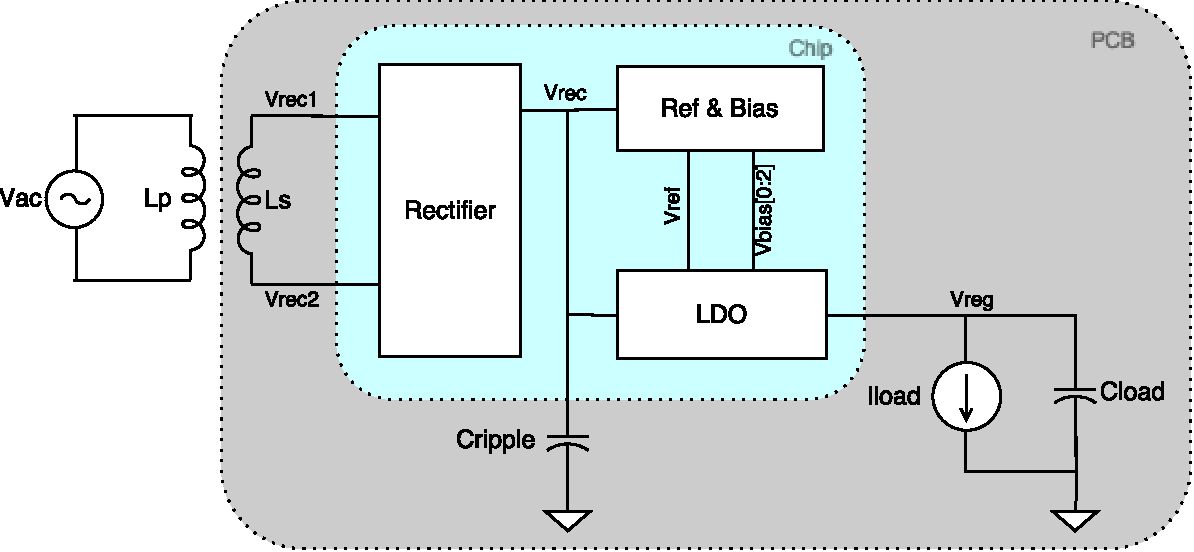
\includegraphics[width=0.8\textwidth]{img/block_diagram.pdf}
   \caption{Block diagram of complete design}
   \label{fig:blockd}
\end{figure}

As shown in the block diagram above, the design includes antennas rectifier, \acrshort{ldo} regulator and reference and biasing circuits. This report mainly discusses about the various design aspect of rectifier and \acrshort{ldo}. The inductor is designed with the specifications provided by NORDIC. The biasing and reference circuit is designed solely for learning the design technique without much effort on the accuracy of the generated biases and references. So externally supplied bias and reference will be the secondary option. The project is designed in tsmc90nm process. Table \ref{proj_spec} lists the main specifications of this project.  \\ 

\begin{table}[!htbp]
\caption{Project specifications}
\begin{center}
\begin{tabular}{c|c}
\hline \hline
Technology & TSMC 90nm CMOS \\ \hline
Chip area & TBA mm\textsuperscript{2} \\ \hline
Vpp for chip & 2.5 V \\ \hline
Max. load & 10 mA \\ \hline
Output dc voltage & 1.8 V \\ 
\hline \hline
\end{tabular}
\end{center}
\label{proj_spec}
\end{table}

A brief discussion of rectifier design is followed next.


\clearpage
\newpage
% *********************************************************************** RECTIFIER  ***********************************************************************

\section{Rectifier}
The most basic rectifier is conventional full wave bridge structure where the diodes are replaced by the diode connected \acrshort{mos}. devices in \acrshort{cmos}. technology. This topology though being simple to implement, has a major drawback. It requires at least twice the $\acrshort{vtn}$ of a MOS device as there are two diode connected MOSes in the conduction path for each cycle of the input signal.  \\

Gate cross coupled and fully gate cross coupled topologies are improvements over conventional full wave rectifier. In gate cross coupled rectifier, two diodes of conventional rectifier is replaced by two gate cross coupled MOSes working as switches where the voltage drop for every cycle is reduced to one threshold voltage. Similarly, in the fully gate cross coupled rectifier, all diodes are replaced by switches and hence the voltage drop is further reduced to twice the conduction drop only for every cycle. Even though this topology has least voltage drop, it suffers from the problem of reverse charge leakage because when the input ac amplitude is less than the output rectified voltage and the conducting pass devices are on simultaneously, current flows backward from output to input. \\

All the above discussed topology suffer from either large voltage drop or large power loss because of which their use are limited in low power and low voltage devices. The popular techniques for higher efficiency are using gate cross coupled rectifier along with passive or active circuitry  for controlling other two pass devices. In passive rectifier, additional circuitry including bootstrap capacitor are used to reduce or eliminate threshold voltage one of which is discussed in this paper \cite{rectboot}. However, use of on-chip bootstrap capacitors limits it use where chip area and speed is of importance. On the other hand, in active rectifier, active circuitry is used control pass devices. The use of active circuitry increase both  \gls{vce} and  \gls{pce} because the pass devices are made to conduct in linear region and hence less conduction drop, and reverse current flow can be completely eliminated and hence less power loss. However active rectifier is not problem free either. The major issue is starting of the active circuit as there is no regulated supply at the start up. \\

In this project, active rectifier is chosen, primarily for better VCE and PCE and secondarily to avoid the use large on chip capacitors. \cite{rectrcc}  and \cite{rectcomp} have discussed same active rectifier topology with a slight difference in active circuitry. \cite{rectrcc} has implemented comparator with compensating the delay of comparator's output falling whereas \cite{rectcomp} has implemented comparator with compensating both the falling and the rising delay of comparator's output in expense of added circuit complexity and power consumption. \cite{rectrcc} has been used here for its simple design. \\

Figure \ref{rect_conv}, \ref{rect_cc} and \ref{rect_rcc} is the CMOS implementation of conventional full wave bridge rectifier, gate cross coupled rectifier and proposed active rectifier in \cite{rectrcc}. The problem with \ref{rect_conv} and \ref{rect_cc} has already been briefly mentioned above. Though  \ref{rect_cc}  is significantly improvement over  \ref{rect_conv} , it is still not a favourable topology with respect to the design technology chosen. In the gate cross couple rectifier of  \ref{rect_cc}, the cross coupled pMOSes act as switches, so the only voltage drop across them is conduction drop due to channel resistance. However the other two nMOSes are diode connected, so they have at least $Vtn$ drop across them which means $Vac \geq Vdc + Vtn$ for conduction.

\begin{figure} [htbp]
  \centering 
  \subfloat[Conventional full wave bridge rectifier]  {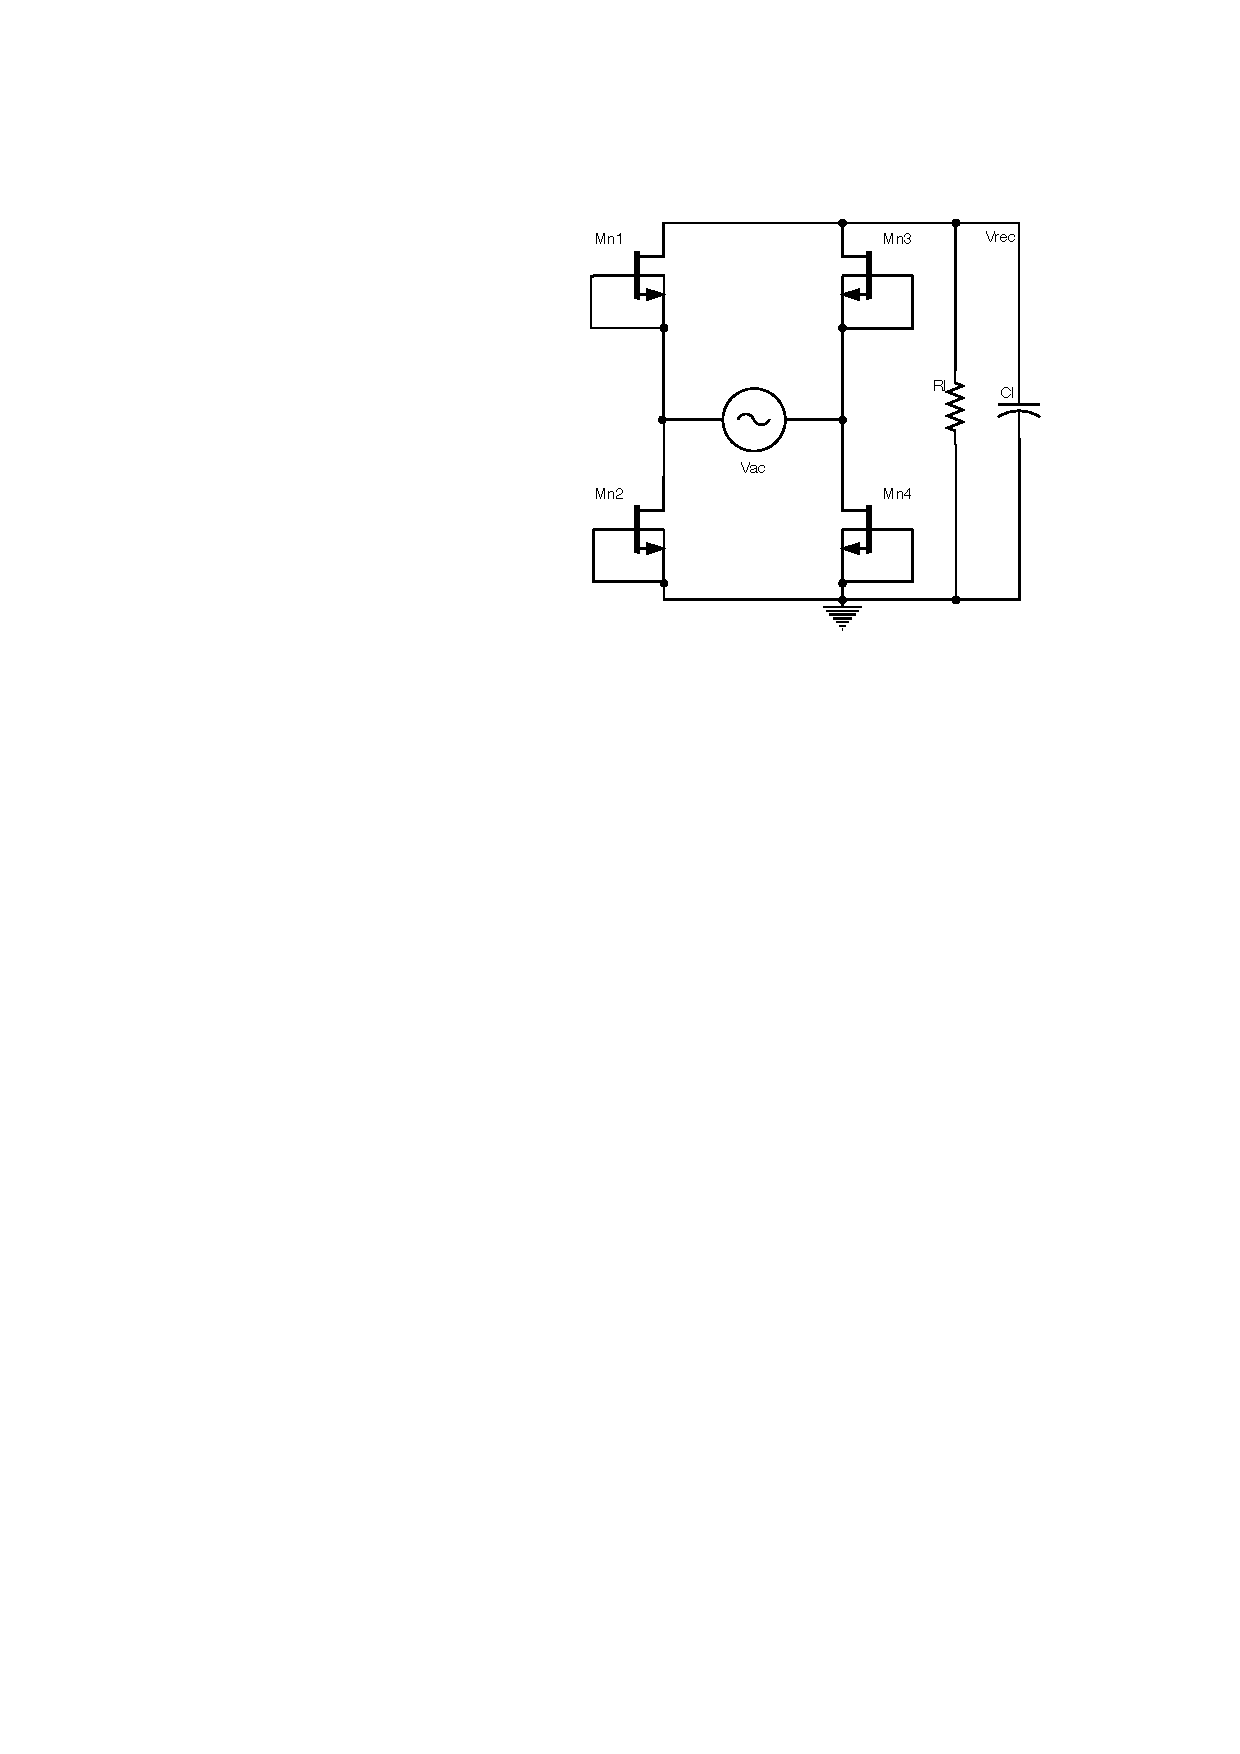
\includegraphics[width=.45\textwidth]{img/rect_conv.pdf} \label{rect_conv}}
\hfill
 \subfloat[Gate cross coupled full wave rectifier]  {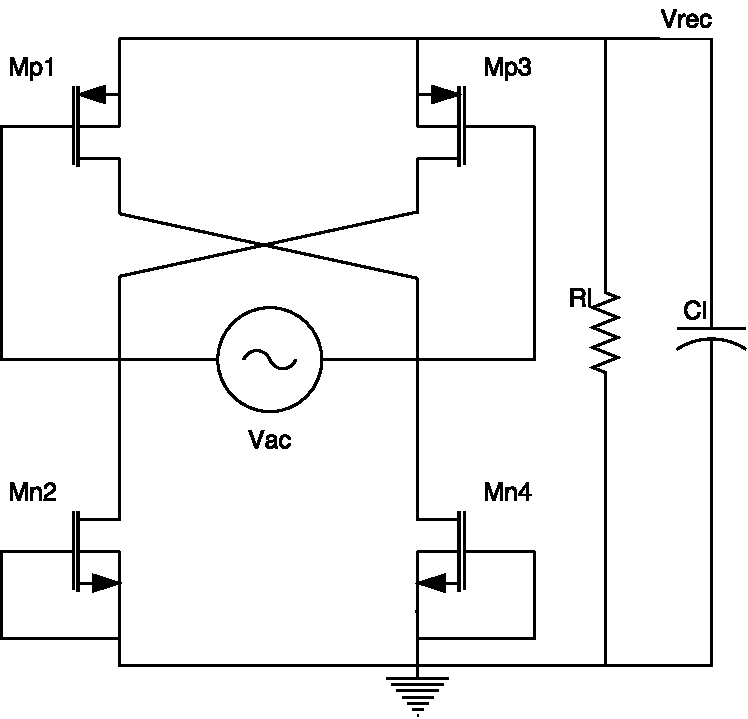
\includegraphics[width=.45\textwidth]{img/rect_cc.pdf}\label{rect_cc}}
 \caption{Rectifier topologies: conventional and gate cross coupled} 
\label{rect_conv_cc} 
\end{figure}

The proposed active circuit in \ref{rect_rcc} is improvement over \ref{rect_cc} which eliminates $Vtn$ drop required for conduction by replacing diode connected nMOS with devices controlled by active circuit as shown in figure \ref{rcc}. The active circuit is a four input comparator that turns on nMOSes fast when Vac > Vdc and turns off fast to avoid flow of current. \\

For the illustration of operation of comparator, consider the case when $Vin1 > Vin2$ i.e. $Vin1 > 0$ and $Vin2 < 0$. During this half cycle, comparator $D1$ output is low and turns off $Mn2$ and also, $Mp1$ is reversed biased and hence there is no path to flow current along $Mn2$ and $Mp1$. For simplicity, assume $Vac =  Vin1 - Vin2$. When $Vac$ reaches $\acrshort{vtp}$, $Mp3$ turns on which shorts $Vin1$ to $Vrec$. When $Vac > Vrec$, $D2$ output goes high, which turns on $Mn4$ and starts the conduction path for the first half cycle and starts charging $Cl$. When $Vac$ reaches maximum, it starts to decrease and at $Vac < Vrec$, conduction stops as output of $D2$ is low and $Mn4$ is off. As $Vac$ further decreases to below $Vtp$, $Mp3$ if off too. This way rectifier in \ref{rect_rcc}  conducts during positive half cycle eliminating the $Vtn$ drop seen in \ref{rect_cc}. Now the only drop is the conduction drop due to channel resistance of two pass devices along the conduction path. This drop is much less because during conduction both the device are operating in the linear region with small resistance. The operation is similar for $Vin2 > Vin1$ where $Mn4$ and $Mp3$ are off and $Mn2$ and $Mp1$ conduct to charge $Cl$. 

\begin{figure} [H]
  \centering 
  \subfloat[Gate cross coupled full wave active rectifer]  {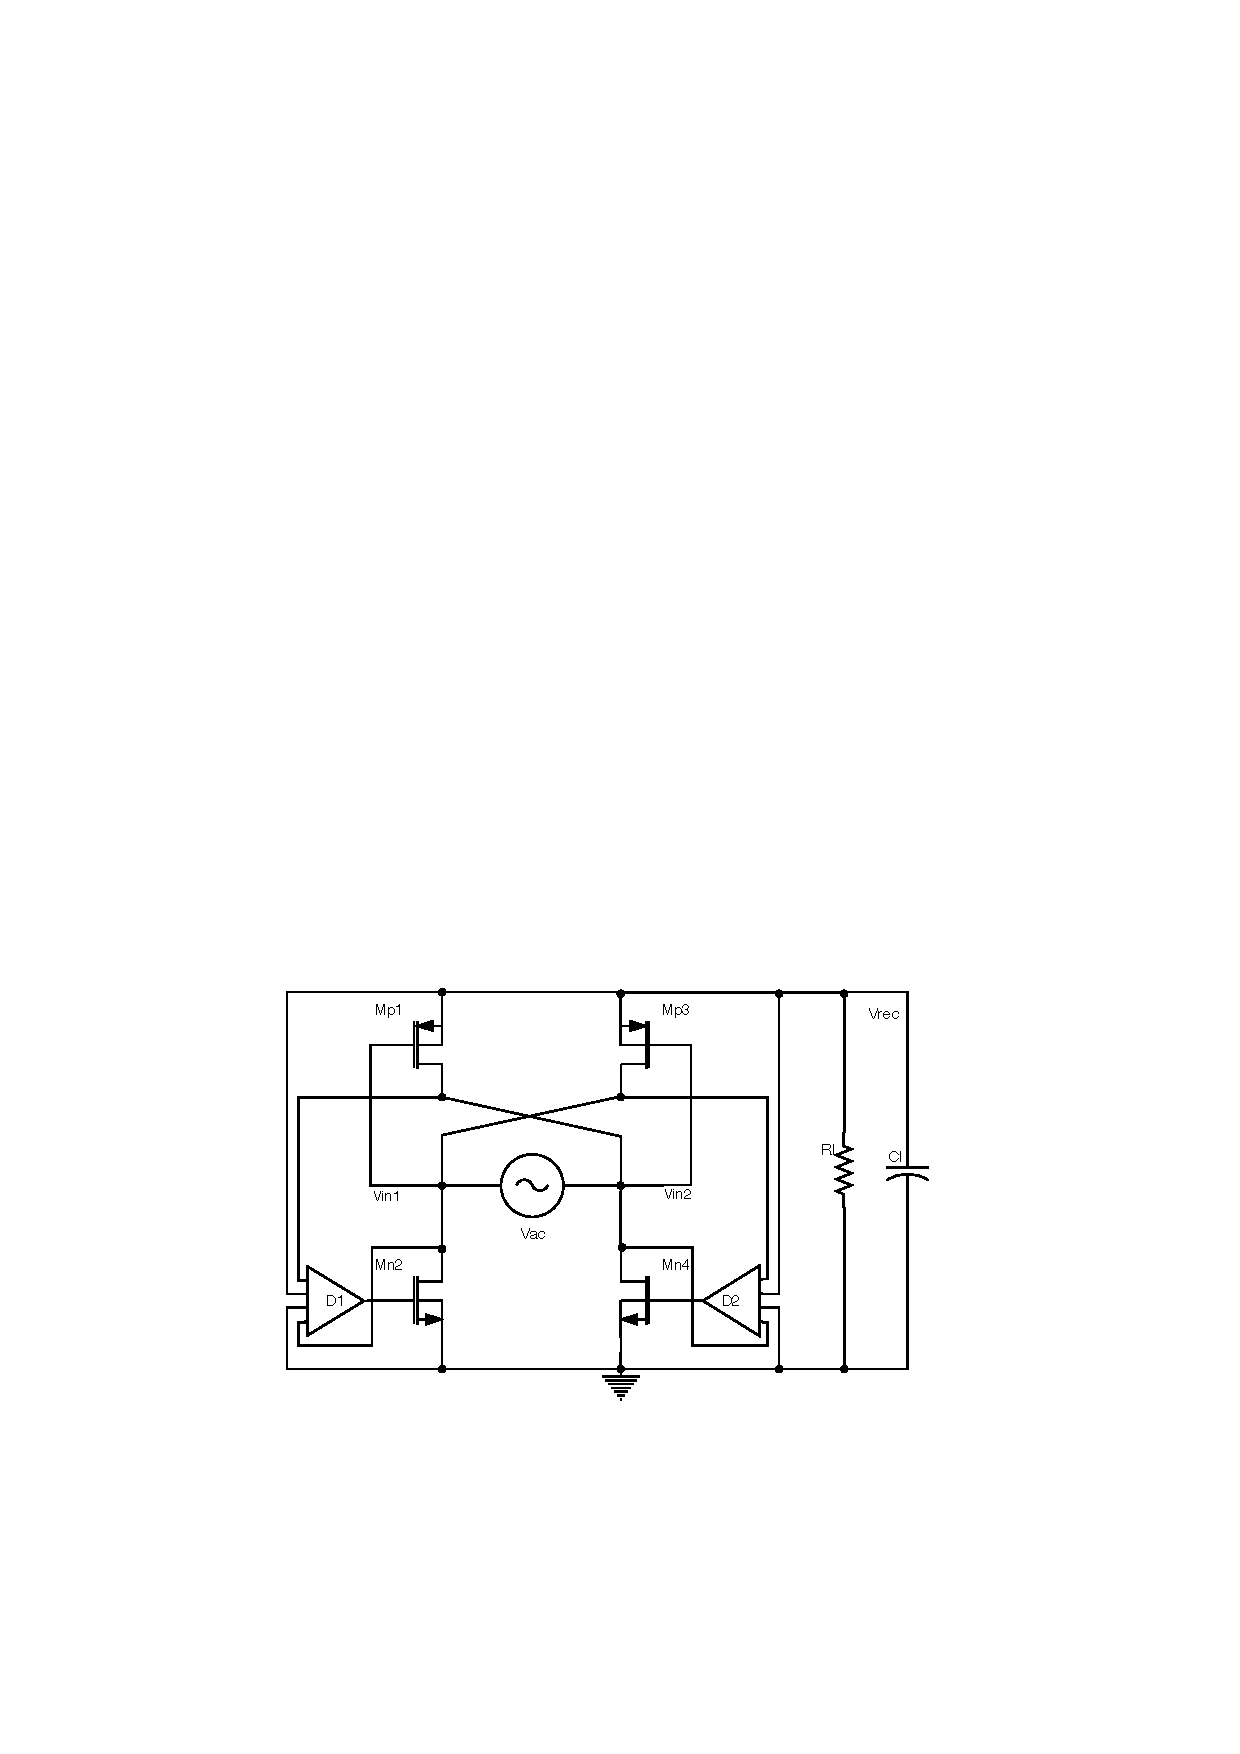
\includegraphics[width=.53\textwidth]{img/rect_rcc.pdf} \label{rect_rcc}}
  \hfill
 \subfloat[Active circuit $D2$]  {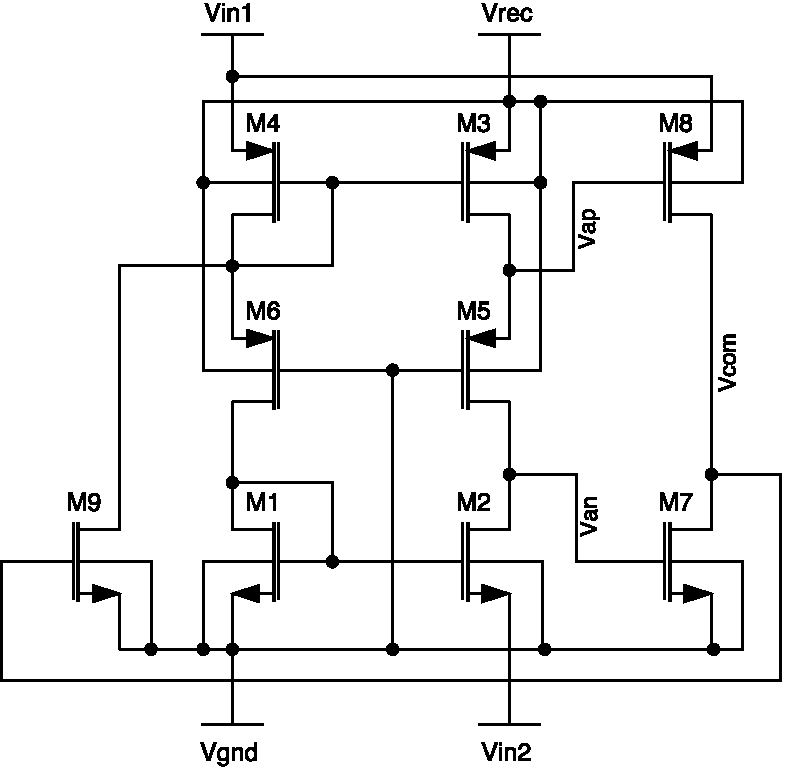
\includegraphics[width=.42\textwidth]{img/rcc.pdf} \label{rcc}}
 \caption{Active rectifier and active circuitry (comparator)} 
\label{rect_rcc_rcc} 
\end{figure}

Figure \ref{rcc}  is the implementation of four input comparator $D2$ used in \ref{rect_rcc} as proposed in \cite{rectrcc}. It is designed to self power and bias because no steady state supply is available at start up. $M1$, $M2$ and $M7$ monitors voltage across $Mn4$ i.e $Vin2 - Vgnd$ and $M3$, $M4$ and $M8$ monitors voltage across $Mp3$ ie $Vin1 - Vrec$ . So when $Vin1 - Vrec > Vin2 - Vgnd$ which means $Vac > Vrec$, output of $D2$ is high and turns on $Mn4$ instantly. But when $Vac < Vrec$, the output of comparator is delayed to fall which causes $Mn4$ to conduct in reverse direction leading to significant reduction in power delivered to load. $M9$ is introduced in order to overcome this problem which adds offset currents to increase $Van$ and $Vpn$ faster, causing the output to decrease faster and turns off $Mn4$ before $Vac < Vrec$. This reverse current control technique compensates the comparator delay and increases the power efficiency of the rectifier. \\

The dimensions of the pass devices are first hand calculated by using square law current equation and devices parameters values given in the technology documents, and later optimised with simulation tool in order to make the rectifier to deliver the required current. Since \acrshort{nmos} does not have to have same device size as \acrshort{pmos} to deliver same current, optimal size ratio equation from \cite{rectsize} is used to find nMOS pass devices sizes.
Similarly, the value of ripple rejection capacitor is chosen 100nF for better ripple rejection at the expense of some additional settling time.

\begin{figure}[htbp] %figure placement: here, top, bottom, or page
   \centering
   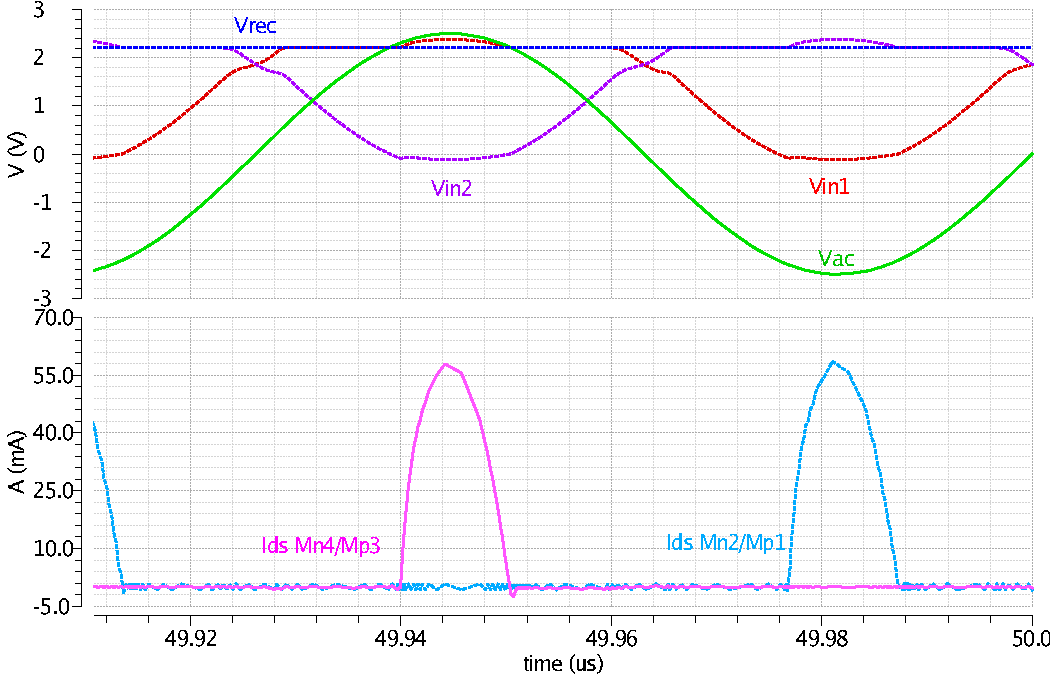
\includegraphics[width=.9\textwidth]{img/rect_output_2.pdf} 
   \caption{Voltage and current waveforms of the rectifier}
   \label{rect_plot}
\end{figure}

Figure \ref{rect_plot} show the simulation results showing voltages and current waveform of this designed rectifier. The generated waveforms clearly follows the working principle discussed above. Two important observations can be made from plots. First, the rectified output $Vrec$ is 2.2 V for $Vpp$ ac input of 2.5 V which means the voltage loss has been significantly reduced and the loss of around 300 mV yields to the conduction loss due the the channel resistance. Secondly, the reverse current from output to input has been effectively eliminated as there is only positive current flowing to the load when all conducting devices are on.  Similarly, figure  \ref{rect_ce} shows PCE and VCE with respect to magnitude peak ac input signal. Both PCE and VCE are very less for input ac amplitude less then 1.8 V. It can be explained by the fact that required bias current and gate drive voltage are not achieved for smaller input. Finally, table \ref{rect_spec} summarises the rectifier design parameters and its performance.

\begin{figure}[htbp] %figure placement: here, top, bottom, or page
   \centering
   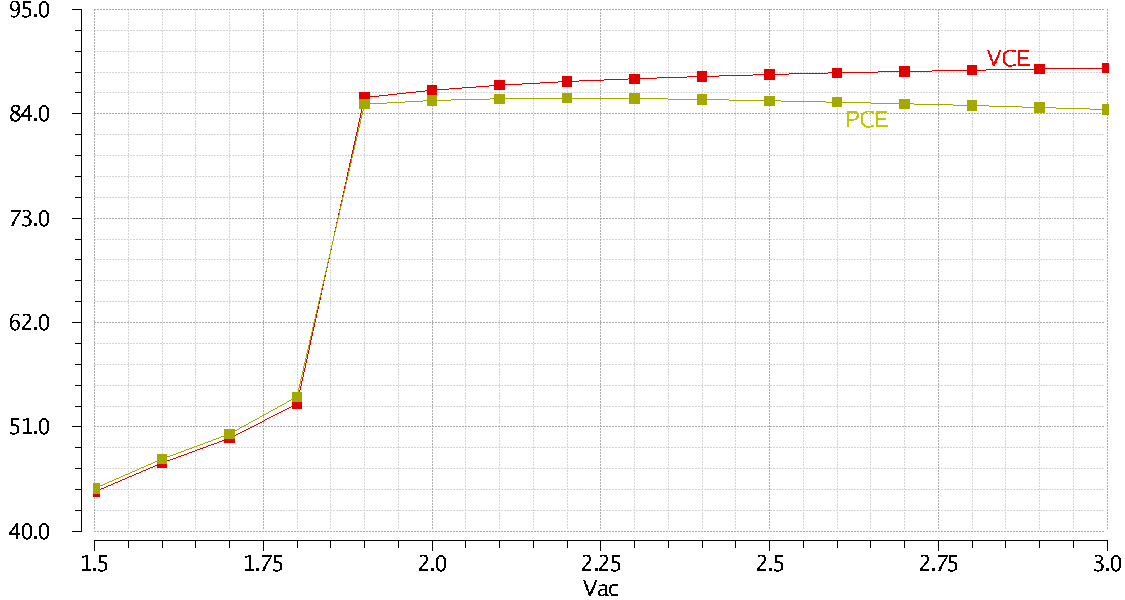
\includegraphics[width=.9\textwidth]{img/rect_ce.pdf} 
   \caption{Voltage and power conversion efficiency}
   \label{rect_ce}
\end{figure}

\begin{table}[H]
\caption{Rectifier parameter and performance}
\begin{center}
\begin{tabular}{c|c}
\hline \hline
Wn/Ln, Wp/Lp & 550um/270nm, 900um/270nm \\ \hline
Rectifier area & TBA mm\textsuperscript{2} \\ \hline
Input ac frequency & 13.56 MHz \\ \hline
Input ac \acrshort{vp} & 2.5 V \\ \hline
Load current & 11 mA \\ \hline
Ripple rejection cap & 100nF \\ \hline
Output dc voltage & 2.2 V \\ \hline
Ripple \acrshort{vpp} & 3 mV \\ \hline
PCE & >85\% \\ \hline
VCE & >88\% \\
\hline \hline
\end{tabular}
\end{center}
\label{rect_spec}
\end{table}


\clearpage
\newpage
% *********************************************************************** LDO  ***********************************************************************

\section{LDO}

Voltage regulator follows the rectifier designed above in order to regulated the rectified voltage to 1.8 V and deliver maximum current of 10 mA. Since the output from the active rectifier is 2.2 V and the required regulated voltage is 1.8 V, charge pump or  \acrshort{smps} of boost type is irrelevant here. Buck SMPS could be an option for voltage regulation but LDO is preferred for it better performance in terms of noise and faster settling of regulated voltage.  \cite{ldo_psu}.\\ 

Figure \ref{ldo_gen} shows a circuit of typical pMOS LDO. As shown in the figure, the components includes an error amplifier (EA), a pass device (Mpass), a feedback circuit (R1 and R2) and load (C\textsubscript{out} and I\textsubscript{load}). A more general and complete LDO circuit also includes the circuitry for generation of reference voltages and bias current/voltages. However, in this project it will be discussed separately for now. In short the working principle of LDO is that the error amplifier compares the scaled down regulated voltage, Vdiv with Vref and regulates the internal resistance of the pass transistor such that  the error, V\textsubscript{ref} - V\textsubscript{div} is least or zero ideally. 

\begin{figure}[htbp] %figure placement: here, top, bottom, or page
   \centering
   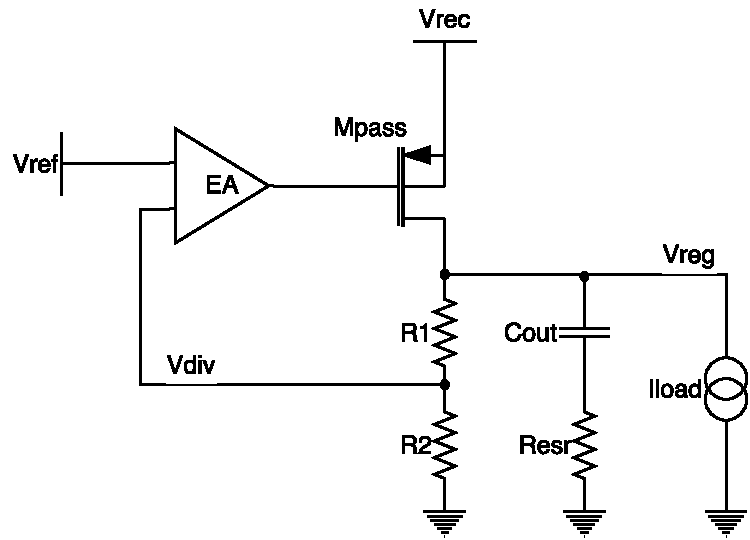
\includegraphics[width=.9\textwidth]{img/ldo.pdf} 
   \caption{Generic LDO with pMOS pass device}
   \label{ldo_gen}
\end{figure}

\cite{ldo_bulkmod} and \cite{ldo_quiescent} are two examples of CMOS implementation of LDO. \cite{ldo_bulkmod} has proposed bulk modulation technique for improving load regulation and stability of capacitor-less LDO. Similarly \cite{ldo_quiescent} has  proposed techniques for increasing current efficiency of LDO especially at no or low load condition. Though the techniques discussed in these designs have not been used, they have given good insight into different design parameters of LDO.  \\

Figure \ref{ldo_cmos} shows the CMOS implementation of LDO in this project. The components in this design include a folded cascode differential amplifier as error amplifier, pMOS buffer, pMOS pass device and feedback network of resistors. 

\begin{figure}[htbp] %figure placement: here, top, bottom, or page
   \centering
   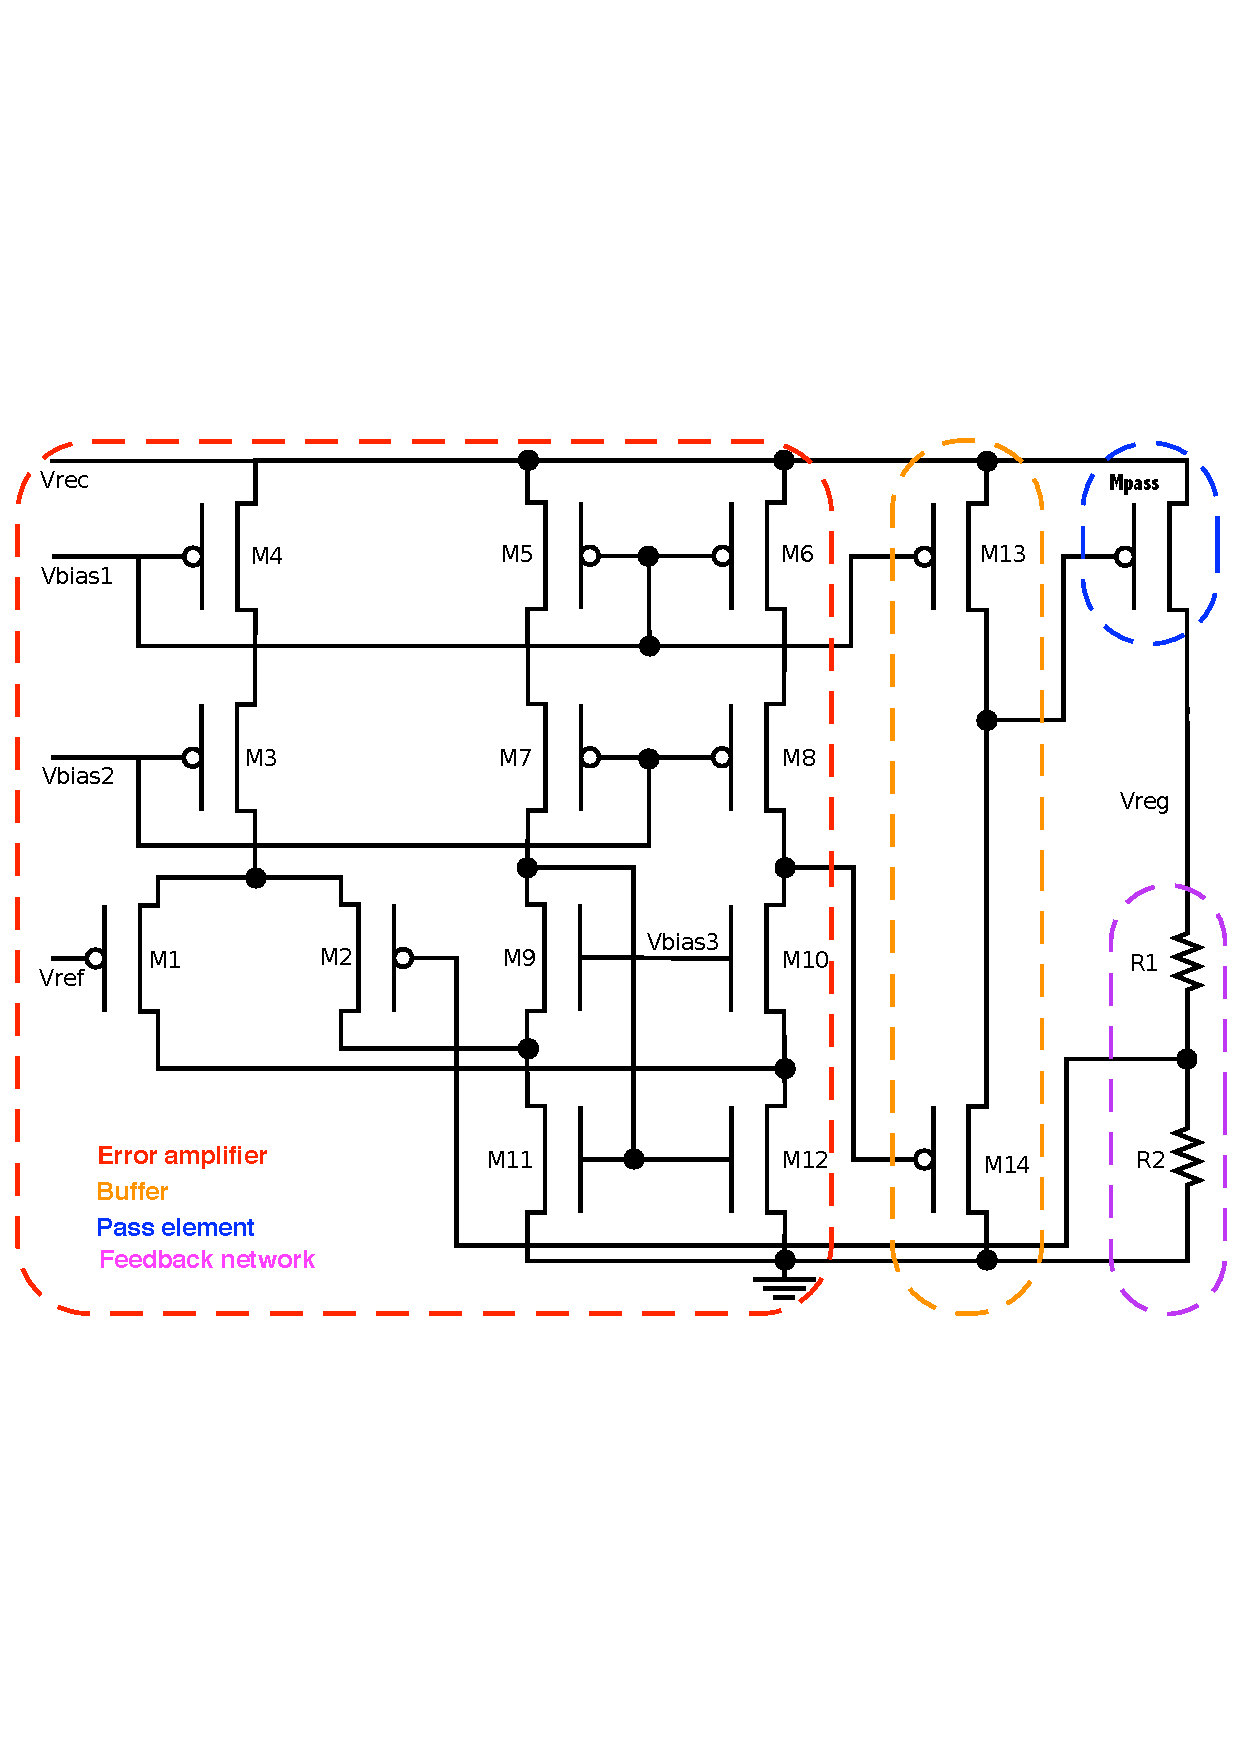
\includegraphics[width=0.9\textwidth]{img/sch_ldo_label.pdf} 
   \caption{CMOS implemenation of LDO}
   \label{ldo_cmos}
\end{figure}

As briefly mentioned above, the error amplifier amplifies scaled regulated voltage, V\textsubscript{div} and reference voltage, V\textsubscript{ref}. It is known that an amplifier with higher open loop \acrshort{dc} gain reduced the closed loop gain error and hence amplifier with higher gain is desired here which is turn increase the accuracy of regulated voltage, Vreg \cite{ldo_bulkmod}. Typically error amplifier has gain $> 40 dB$ which is not achieved with the single stage amplifier with this technology. Higher gain could have been achieved with multiple single stage but with increased difficulty in making the amplifier stable. So for achieving higher DC gain and at the same time for stability convenience, folded cascode amplifier \cite[pp. xx]{razavi_2001} is chosen. \\

The amplifier has a pMOS differential input stage in order to obtain lower \acrshort{icmr} of the amplifier closer to gnd because so is V\textsubscript{ref}. In addition, this helps in pushing the poles at the folding point farther, easing the stability of the amplifier\cite[pp. 304-305]{razavi_2001}. Similarly, a pMOS buffer is used to supply sufficient current to drive the large pass transistor.  Moreover, pMOS as buffer passes 1 better which means it can turn off the pass device completely and hence LDO regulates better at low load or no load condition. However at heavy load/large load current, the pMOS buffer is not able to pull down the gate of pass device as low as possible.  This is overcome by making the pass device large enough to feed the required load current.\\

The pass device is a pMOS transistor in this design. It is chosen because it has several advantages over it's counterparts like nMOS and BJT devices in terms of dropout voltage, quiescent current, input voltage, thermal response and noise\cite{ldo_ti_pmos}. Prominently, there are two factors that give pMOS edge over other devices; dropout voltage and quiescent current, when it comes to application in low power and low voltage devices. nMOS as a pass device requires a positive drive voltage with respect to output to operate. On the other hand, pMOS is driven by a negative signal with respect to input which means pMOS is preferable for a low input LDO. Similarly compared to BJTs, pMOS requires less headroom and less quiescent current to be driven\cite{ldo_ti_pmos}, \cite{ldo_ti_stability}, which means low dropout and low power operation, typical requirement of today's micro devices' power supply. \\

However, pMOS as a pass device in LDO causes challenges in stability. As mentioned above, LDO utilises a high gain feedback loop in order to provide a regulated output voltages independent of load current and in any system with feedback loop, the locations of poles and zeros determine stability of the system.  In case of the pMOS LDO, the pass device is configured in a common source configuration. LDO with big output cap has a dominant pole pole at the output, which is a low frequency pole. The second pole is located at the gate of pass device because as mentioned earlier pMOS pass device is large and has a big parasitic capacitance. This second pole may be located closer to the dominant pole, resulting in significant  reduction in phase margin (\acrshort{pm}). Consequently, this may lead to instability of the LDO with pMOS pass device.  Various methods have been implemented for ensuring the stability of the pMOS LDO. In this project, a large external capacitor, $C\textsubscript{load}$ in figure \ref{ldo_gen}, is used for stabilising the system at the cost of additional settling time. When an external capacitor is used for designing a stable LDO, the minimum value of capacitance, $C\textsubscript{load}$ and minumum value of its equivalent series resistance (\acrshort{esr}), $R\textsubscript{esr}$ should be specified\cite{ldo_ti_stability}. $C\textsubscript{load}$ determines the dominant pole of the LDO and $R\textsubscript{esr}$ in series with $C\textsubscript{load}$ introduces a left half plane zero below unity gain frequency(\acrshort{ugf}) of LDO in order to cancel out the non-dominant pole below UGF, producing a stable LDO system. \\

\begin{figure}[htbp] %figure placement: here, top, bottom, or page
   \centering
   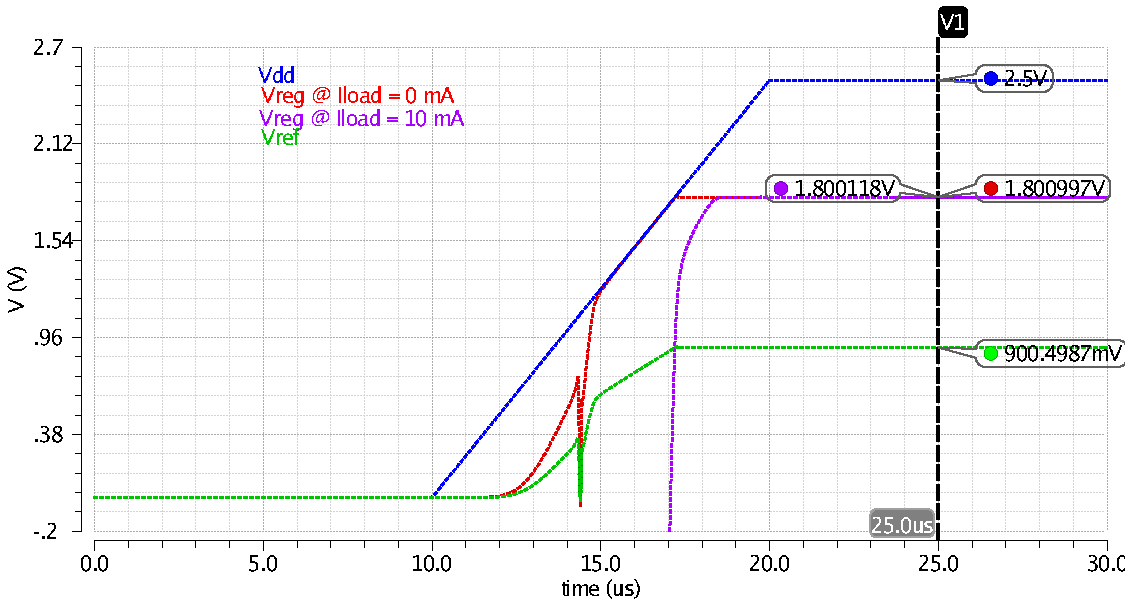
\includegraphics[width=0.9\textwidth]{img/ldo_tran.pdf} 
   \caption{LDO transient simulation}
   \label{ldo_tran}
\end{figure}

Figure \ref{ldo_tran} is the transient simulations of the LDO which illustrates the generation of $Vreg$ for both high load and no load condition. This waveforms show that once the $Vdd$ reaches high enough to create proper biasing, the regulated voltage of 1.8 V is produced and remains constant henceforth.

\begin{figure}[htbp] %figure placement: here, top, bottom, or page
   \centering
   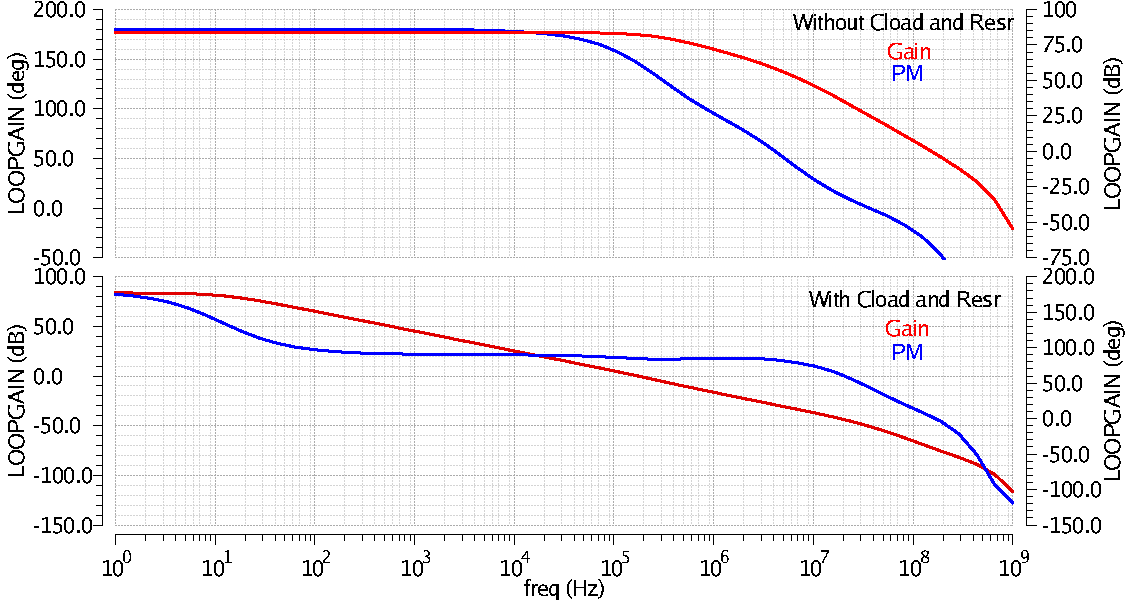
\includegraphics[width=0.9\textwidth]{img/ldo_sta.pdf} 
   \caption{LDO stability before and after compensation}
   \label{ldo_sta}
\end{figure}

Figure  \ref{ldo_sta} the gain open loop gain and phase margin of LDO without (upper plot) and with (lower plot) compensation. Though the stability analysis plots shown above is for typical corner of the devices, the values of $R\textsubscript{esr}$ and $C\textsubscript{load}$ are chosen for PM of at least 45\textdegree  for the worst case i.e. slow corner and maximum load condition. \\ 

\begin{table}[H]
\caption{LDO parameter and performance} 
\begin{center}
\begin{tabular}{c|c}
\hline \hline
(Wp/Lp)\textsubscript{pass} & 240um/280nm \\ \hline
Input supply voltage & 2.2 V \\ \hline
Regulated output voltage & 1.8 V \\ \hline
I\textsubscript{load} max. & 10 mA \\ \hline
C\textsubscript{load} min. & > 0.6 \si{\micro\farad}  \\ \hline
R\textsubscript{esr} min. & > 0.8 $\Omega$ \\ \hline
PM & 84\textdegree (typical) \\ %\hline
%Load regulation & TBA\\ \hline
%Line regulation &    TBA \\ 
\hline \hline
\end{tabular}
\end{center}
\label{ldo_spec}
\end{table}%

Reference and biasing circuit design follows next. \\


\clearpage
\newpage
% *********************************************************************** REFERENCE AND BIASING  ***********************************************************************

\section{Reference and biasing}

Reference and biasing circuit is important part of any analog circuit. It is required to bias the designed circuitry with proper voltages and currents for operating all the devices in the intended region. For reliable and consistent  performance of the system, the references and biases should be independent of supply voltage and temperature variations. Moreover with the trend of shrinking device sizes, mismatch and process parameters variations have been so pronounced that these factors affect the operation of the devices. So for the todays' devices, it is necessary to design reference and biasing independent of \acrshort{pvt} variations. \\

There are different methods of generating reference voltages and bias currents discussed in literatures. Basically, supply independent current source is generated first and then this current is passed through a resistor to get a reference voltages. Some ways of creating supply insensitive current sources are threshold voltage referenced, diode ($V_{BE}$ in BJT) referenced thermal voltage referenced current sources \cite[pp. 305-315]{gray_2009}. However, these current sources are not temperature independent. Threshold voltage of MOS and forward voltage of diode or $V_{BE}$ have a negative temperature coefficient \acrshort{tc}  and hence they produce a \acrshort{ctat} (complementary to absolute temperature) current. On the other hand, the thermal voltage($V_T$) has positive TC and hence it produce a \acrshort{ptat} (proportional to absolute temperature) current. So these techniques, though being insensitive to supply variations, still cannot be used for accurate reference voltage generation because of temperature dependence. So \gls{bgr} design is used to generate the required reference voltage for the LDO in this design which has significantly less PVT variations than the last three methods.\\

BGR design involves summing up two voltages of which one is PTAT and the other is CTAT, both having equal and opposite TCs. The equal and opposite TCs cancels out leaving the resultant voltage with a zero TC. Figure  \ref{bgr_sch} is the CMOS implementation of reference and biasing circuit for this project which includes startup circuit, BGR circuit and biasing circuit. \\

\begin{figure}[htbp] %figure placement: here, top, bottom, or page
   \centering
   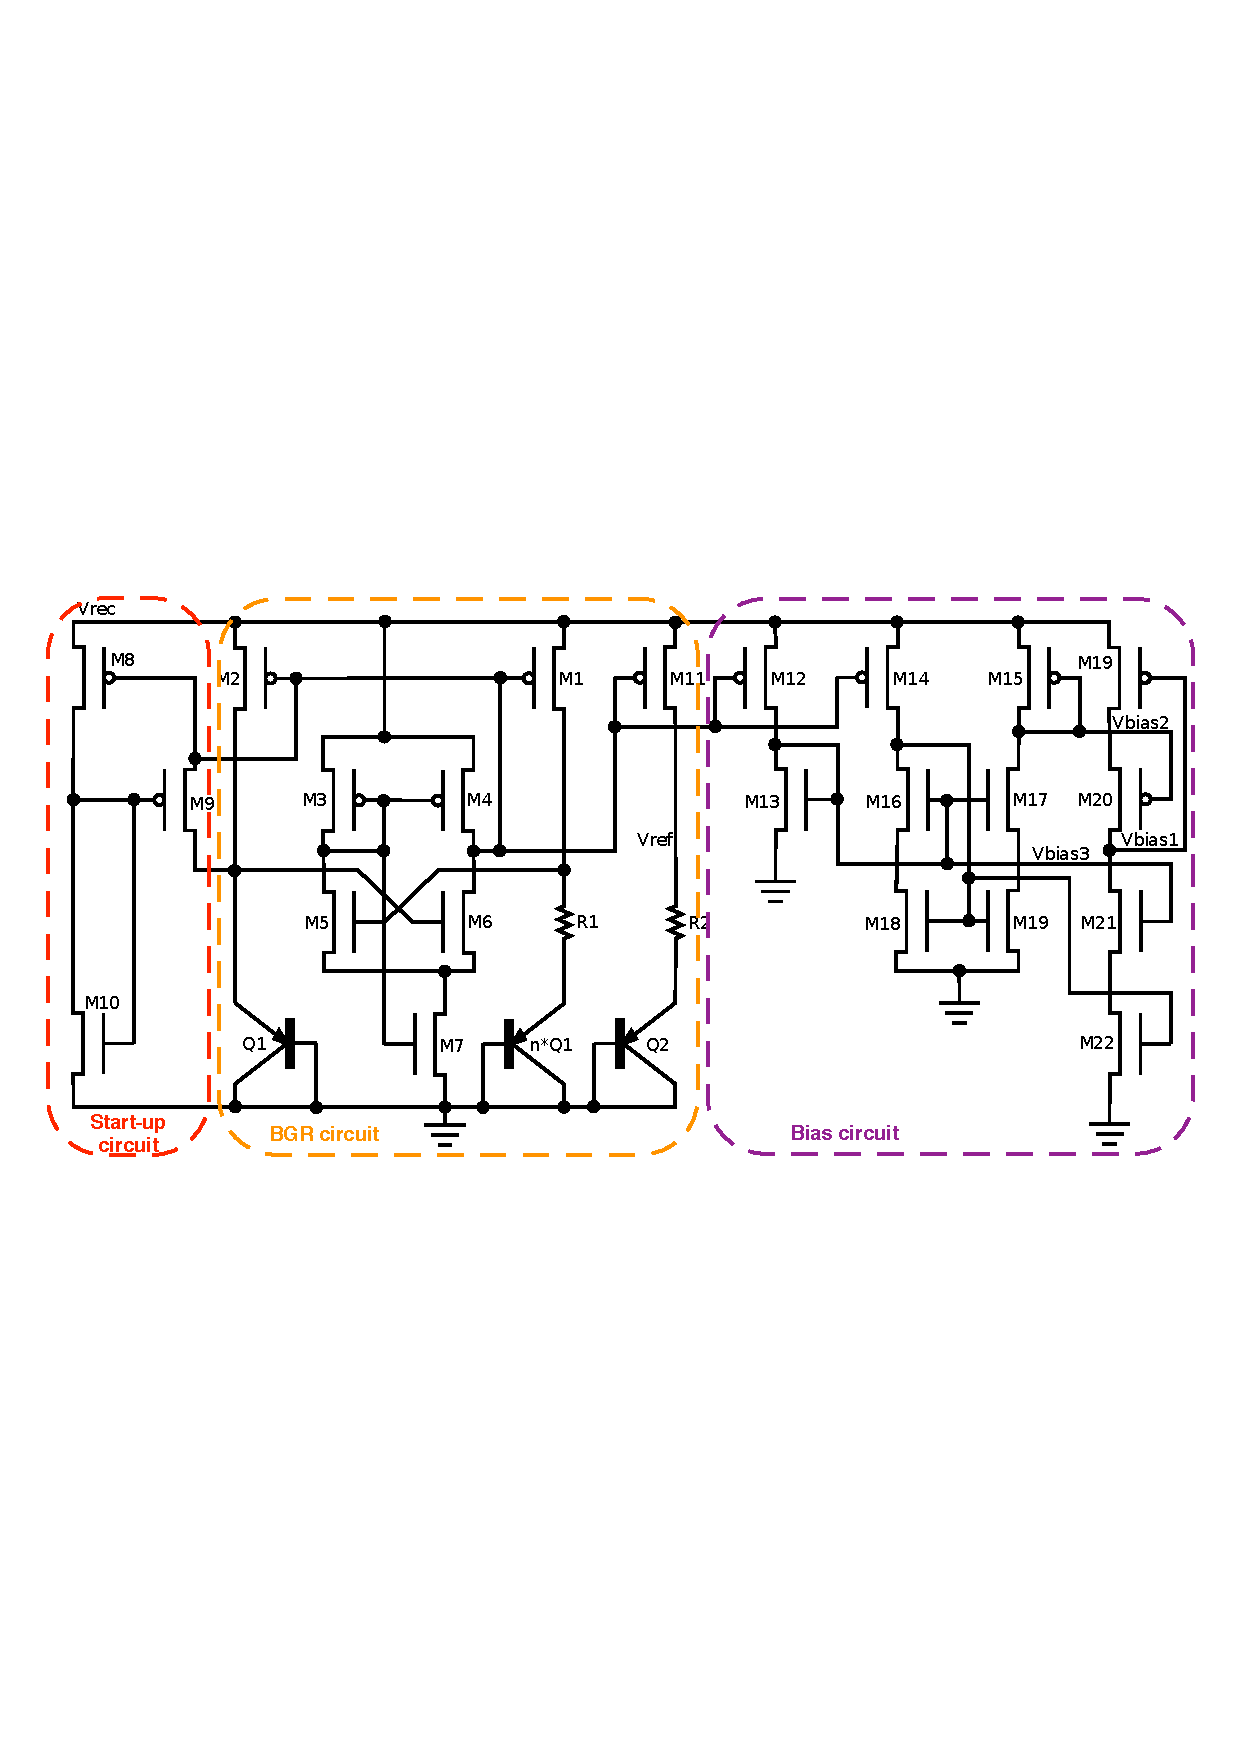
\includegraphics[width=\textwidth]{img/sch_bgr_label.pdf} 
   \caption{BGR and bias generation circuit}
   \label{bgr_sch}
\end{figure}

PTAT current is first generated using thermal voltage referenced current source using PNP transistor as diodes, resistor and a op-amp controlled current mirror \cite[pp. 391-392]{razavi_2001}. The current is $I = V_T ln(n)/R_1$, where $V_T = kT/q $ is thermal voltage with positive TC and $n$ is number of parallel PNP transistors. This current is passed through a resistor, $R_2$ to create a PTAT voltage which is in series with a diode realised with a parasitic PNP transistor. The value of $R_2$ is so chosen such that the positive TC of PTAT voltage across it is equal to negative TC of $V_{BE}$. The temperature independent reference voltage is then given as $V_{ref}  = V_{BE} + \alpha V_T ln(n)$, where $ \alpha = R_2/R_1$ is equal to $  \Delta V_{BE}/\Delta T$. Similarly the folded cascode  \gls{ota} working as an error amplifier in LDO requires additional bias voltages which are produced as shown. Wide swing current mirror topology is used here for bias voltage generation.\\

In case of the supply independent and self biased circuit, there may be start-up issue. If all the transistors carry zero current, they may indefinitely remain off even when the supply is turned on. Therefore start-up circuit is added in order to ensure that the devices are turn on as supply voltage is provided. Once the circuit is fully operational, the start-up circuit is off and does not effect the normal operation of BGR circuit. \\

Figure  \ref{bgr_temp}, \ref{bgr_dc} and \ref{bgr_tran} illustrates temperature, DC and transient simulation of the BGR circuit respectively for slow(ss), fast(ff) and typical(tt) corners. The plots shows that $V_{ref}$ is fairly independent with PVT variations. Similarly, $I_{bias}$ varaitons used for generating the bias voltages remains within condiderable range. Table \ref{bgr_spec} summarizes the performances of the BGR design. 

\begin{figure}[htbp] %figure placement: here, top, bottom, or page
   \centering
   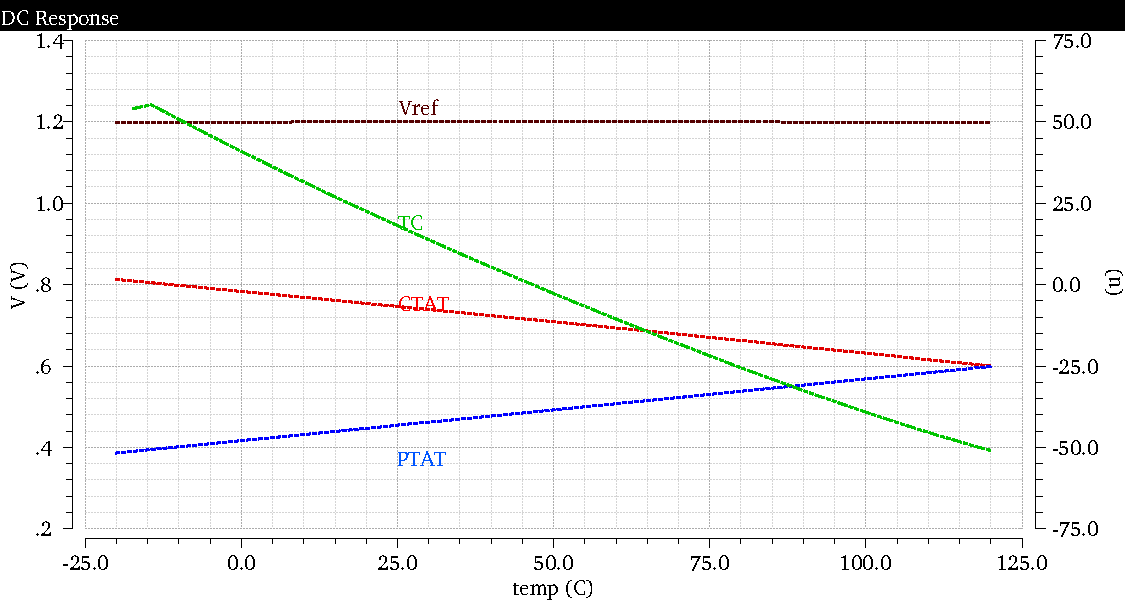
\includegraphics[width=0.9\textwidth]{img/bgr_temp.pdf} 
   \caption{BGR over temperature varitaion}
   \label{bgr_temp}
\end{figure}

\begin{figure}[htbp] %figure placement: here, top, bottom, or page
   \centering
   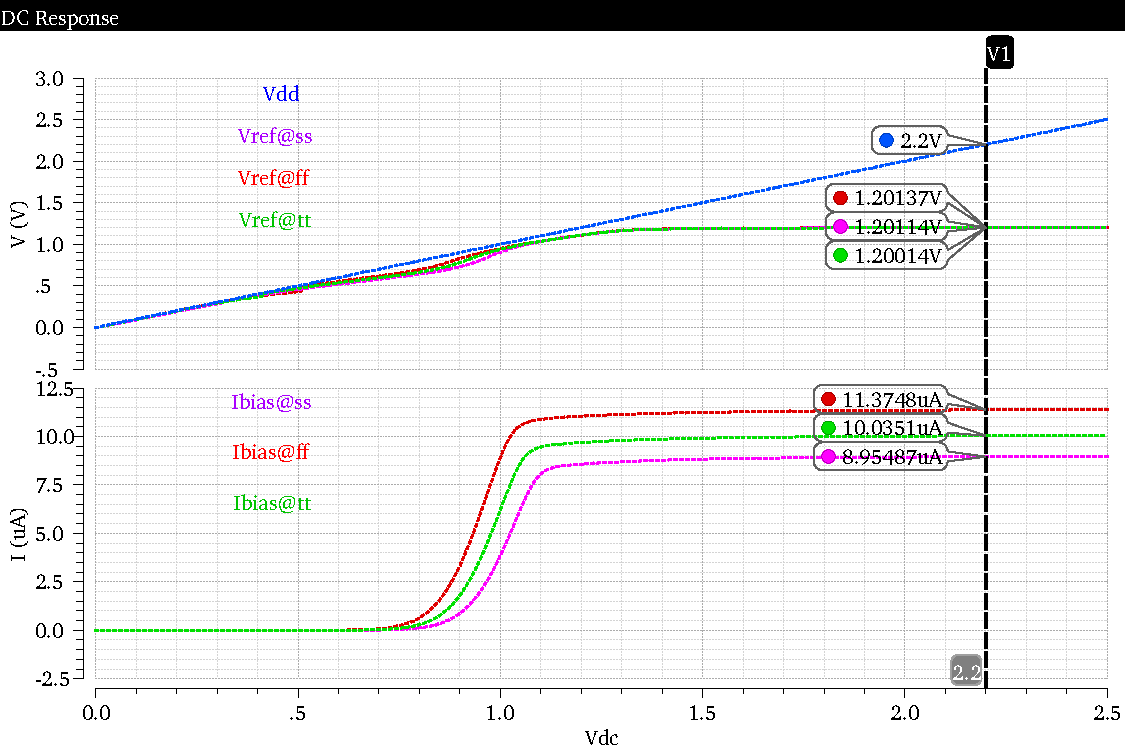
\includegraphics[width=0.9\textwidth]{img/bgr_dc.pdf} 
   \caption{BGR DC performance}
   \label{bgr_dc}
\end{figure}

\begin{figure}[htbp] %figure placement: here, top, bottom, or page
   \centering
   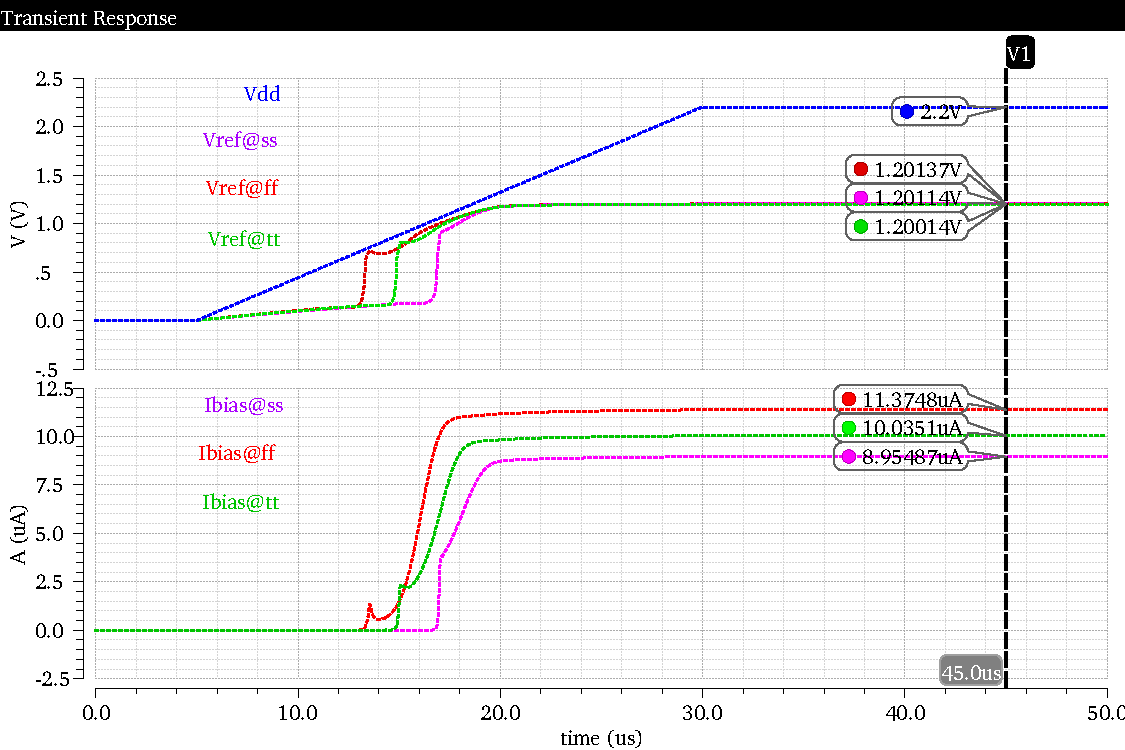
\includegraphics[width=0.9\textwidth]{img/bgr_tran.pdf} 
   \caption{BGR transient performance}
   \label{bgr_tran}
\end{figure}

\begin{table}[htbp]
\caption{BGR parameter and performance}
\begin{center}
\begin{tabular}{c|c}
\hline \hline
\multirow{3}{*}{V\textsubscript{ref}} & 1.201.1 \si{\volt} @slow corner \\ \cline{2-2}
& 1.201.4 \si{\volt} @fast corner \\ \cline{2-2} %\hline
& 1.200.1 \si{\volt} @typical corner \\ \hline
TC @27\textdegree C & 16.4 \si{\micro\volt}/\textdegree C \\ \hline
\multirow{3}{*}{I\textsubscript{bias}} & 8.95 \si{\micro\ampere} @slow corner \\ \cline{2-2}
& 11.37 \si{\micro\ampere} @fast corner \\ \cline{2-2}
& 10.04 \si{\micro\ampere} @typical corner \\ 
\hline \hline
\end{tabular}
\end{center}
\label{bgr_spec}
\end{table}%


\clearpage
\newpage
% *********************************************************************** ANTENNA DESIGN  ***********************************************************************

\section{Antenna Design}

All the components discussed above are part of any power management system. However, it is  a pair of 
antennas which created inductive links for transferring power wirelessly and hence it is the actual physical 
component which makes wireless power transfer possible. \\


As already stated inductive coupling means coupling one coil with other, through magentic field created in the 
first coil which induces the voltage in the second one. This is exactly the phenomenon for creating wireless 
power transfer link. In this project, the antenna dimesnions are provided by Nordic Semiconductor which is one 
of their design already used in some application. Since having similar shape and size of antennas is important 
in gaining more transfer efficiency, the same antenna type is used as both primary and secondary coils. \\


For purpose of this work, with provided dimensions of the antenna, it is first modelled in HFSS as shown in 
figure \ref{fig:ant_single_model}. To realise a real antenna, physical parameters of materials used for making 
printed antenna on a PCB are also given for the model.  After completing model, frequecny sweep is done for extracting S parameter of the 
antenna which was eventually used to estimate  self inductanace of the modelled coil. The performance estiamtion of 
single antenna here and couple system later is based on formulas in \cite{ant_SZ_formula}. In order to check and compare the estimated inductance value from 
the model, two different mathematical approximation methods described in \cite{ant_inductance_calculation} were used. All the values of 
inductance of the antenna estimated from different method is listed in table \ref{tab:ant_inductance_compare}. The table shows that the 
modelled value is less than mathematically approximated values. This difference can be explained with two things. 
Firstly, mathematical calculation assumed that the antenna is spiral and rectangular with sharp edge but the model has 
rounded edge. Secondly, during modelling besides dimesnions of the coils, physical parameters of coil materials are also used 
but these are not considered for mathematical calculation.\\

\begin{figure} [!htbp]
  \centering 
  \subfloat[HFSS antenna model]  {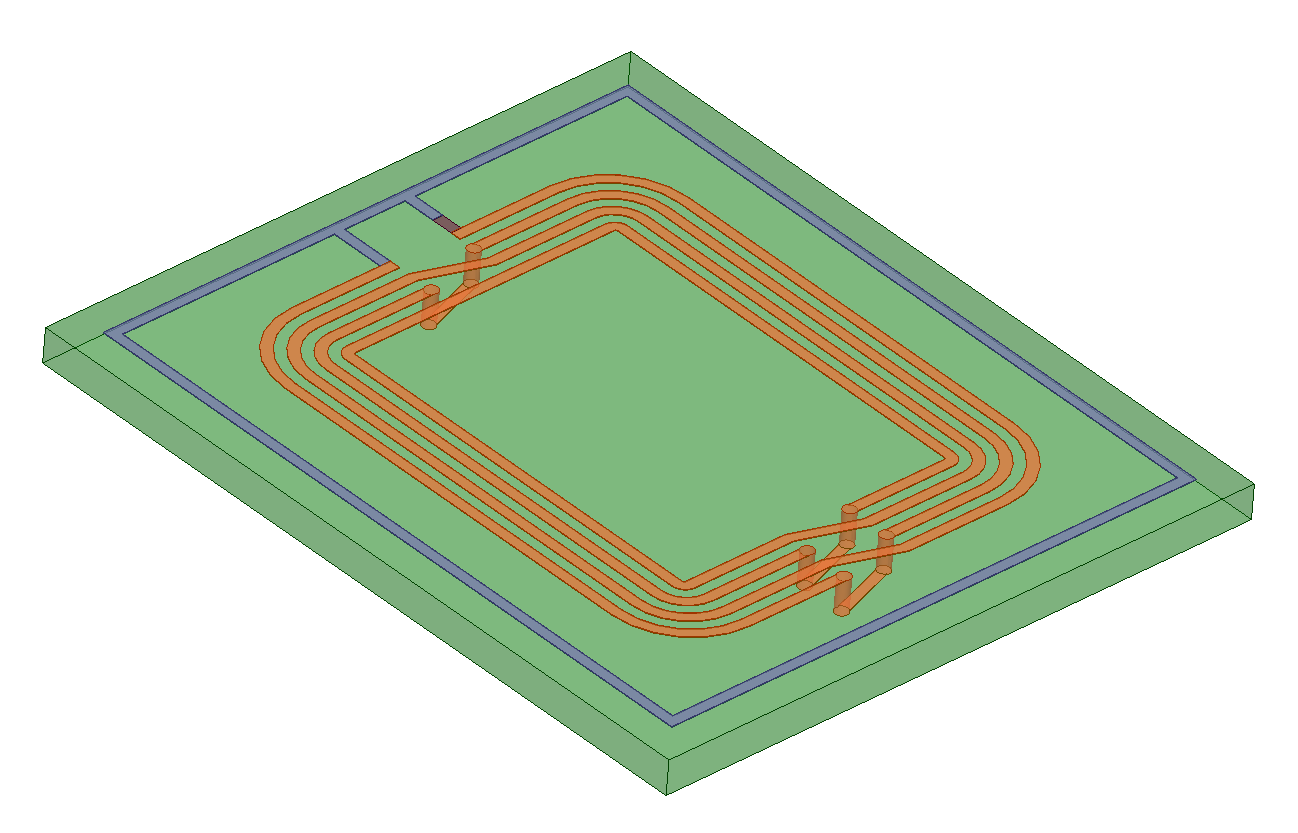
\includegraphics[width=.49\textwidth]{img/ant_single.png} \label{fig:ant_single_model}}
\hfill
 \subfloat[Equivalent schematic]  {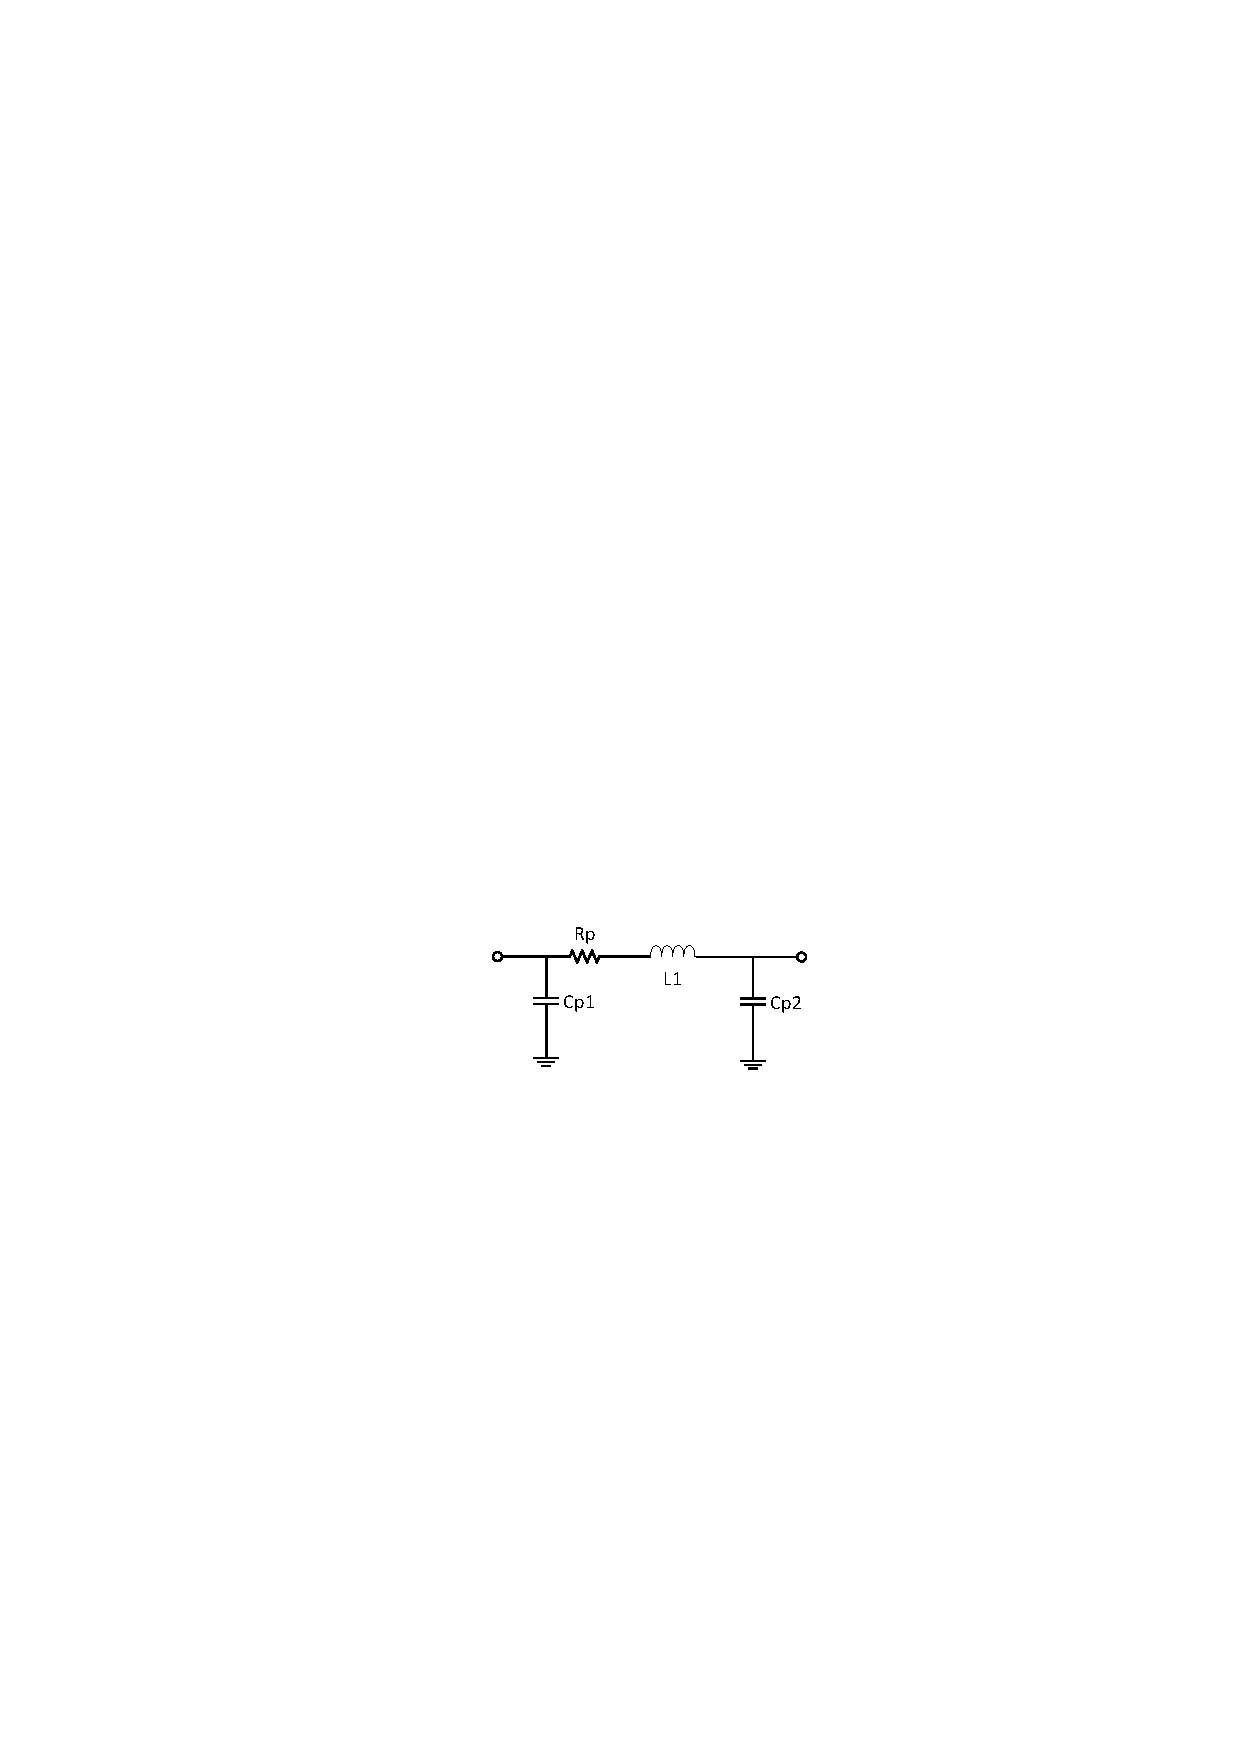
\includegraphics[width=.49\textwidth]{img/ant_single.pdf}\label{fig:ant_single_schematic}}
 \caption{Antenna model} 
\label{fig:ant_single} 
\end{figure}

\begin{figure}[!htbp] %figure placement: here, top, bottom, or page
   \centering
   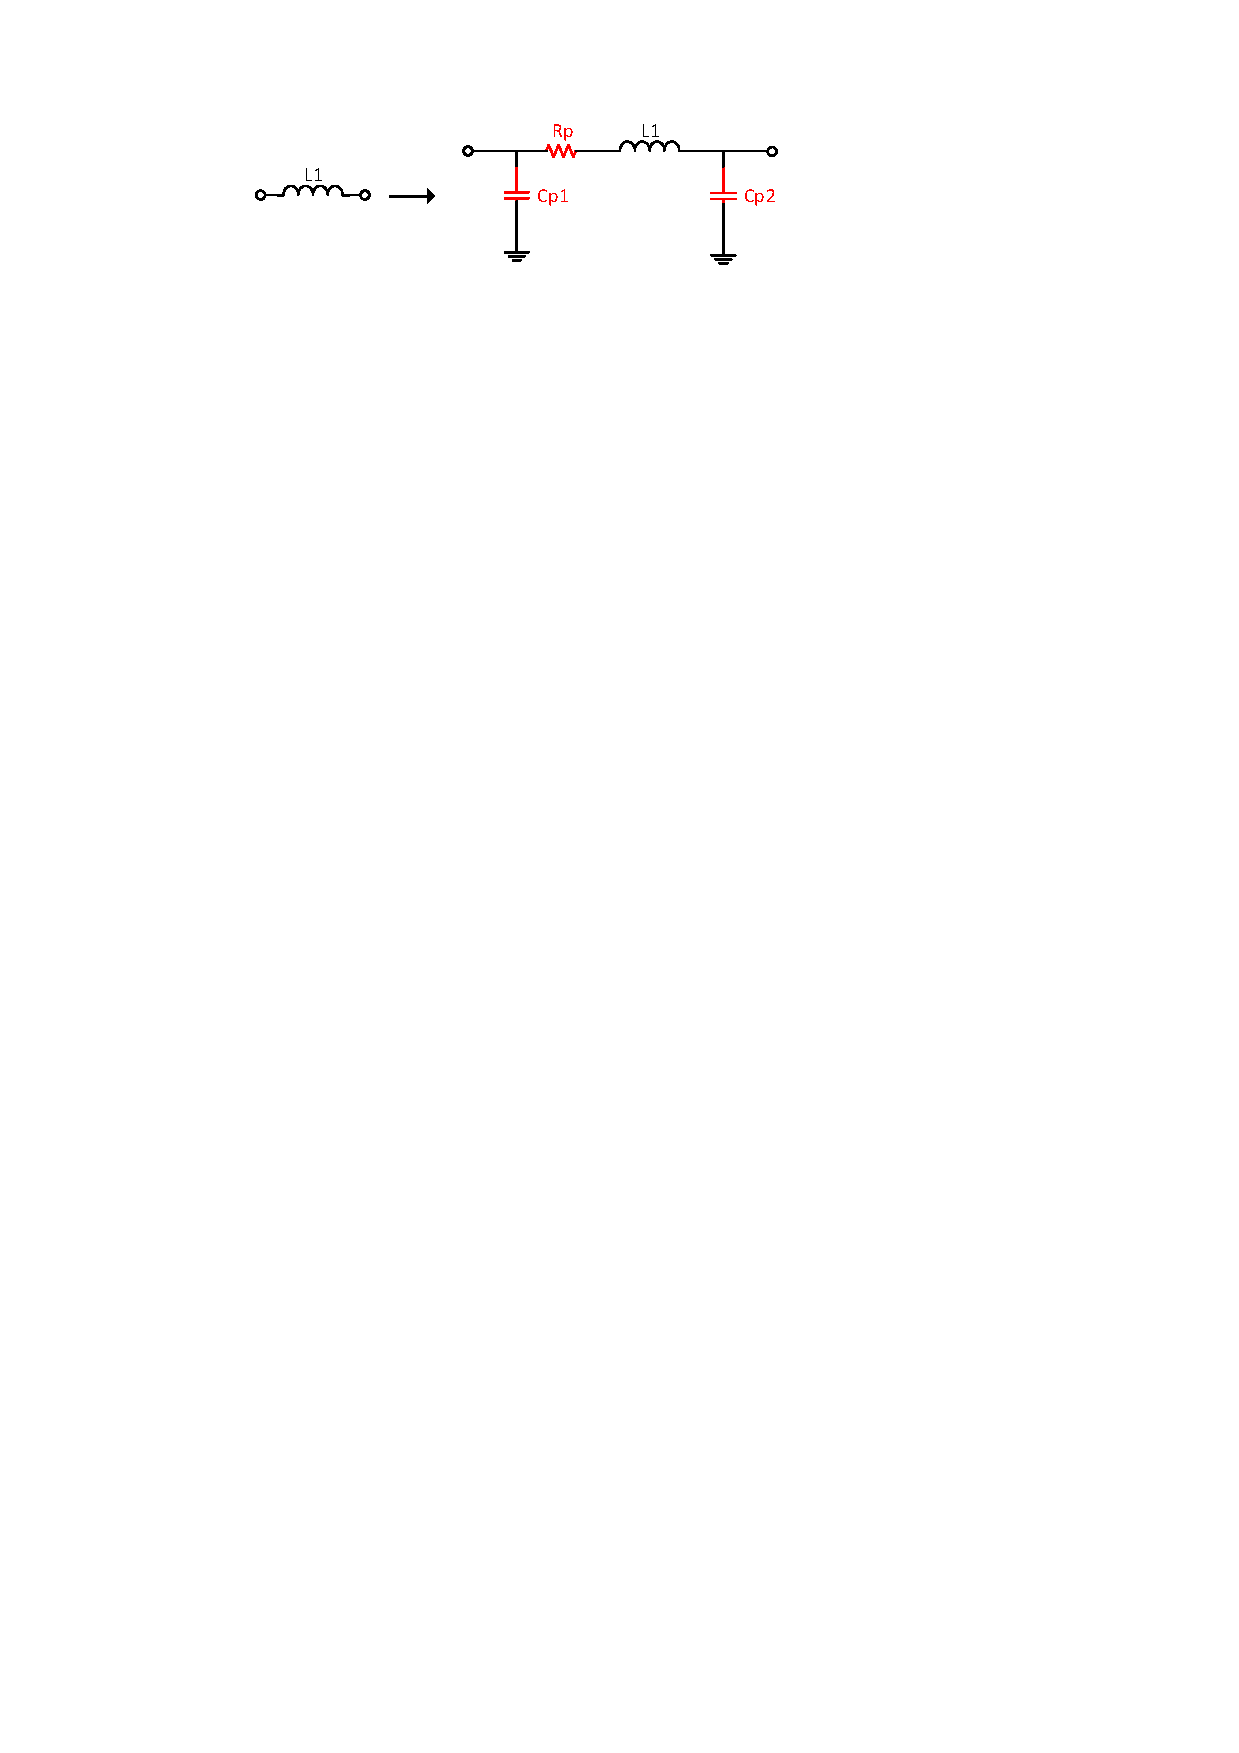
\includegraphics[width=0.6\textwidth]{img/ant_non_ideal.pdf} 
   \caption{Real antenna model schematic}
   \label{fig:ant_non_ideal}
\end{figure}

\begin{table}[H]
\caption{Self inductance estimates comparision} 
\begin{center}
\begin{tabular}{c|c}
\hline \hline
HFSS model extraction & 448 \si{\nano\henry} \\ \hline
Modified Wheeler Formula \cite{ant_inductance_calculation} & 644 \si{\nano\henry}  \\ 

\hline \hline
\end{tabular}
\end{center}
\label{tab:ant_inductance_compare}
\end{table}%

The next step is to observe coupling of two antenna for varying distance of field interaction. Two coils, primary 
and secondary are aligned together sepatated by some distance as shown in \ref{fig:ant_couple}. The same procedure as 
used for single coil above, is used to extract self inductance of each coil, $L1$ and $L2$, mutual inductance 
of two coils, $L12$, coupling cofficient between the coils, $k$ and quality factor, $Q$. The extracted values for coil separtaion of 
1mm, 5mm and 10mm are listed in table \ref{tab:ant_couple_parameter}. $L1$ and $L2$ are same as in 
table \ref{tab:ant_inductance_compare} as it is the same coil used as primary and secondary. Similarly $L12$ and 
$k$ are both decreasing with distance as expected.\\

\begin{figure} [htbp]
  \centering 
  \subfloat[HFSS coupling model]  {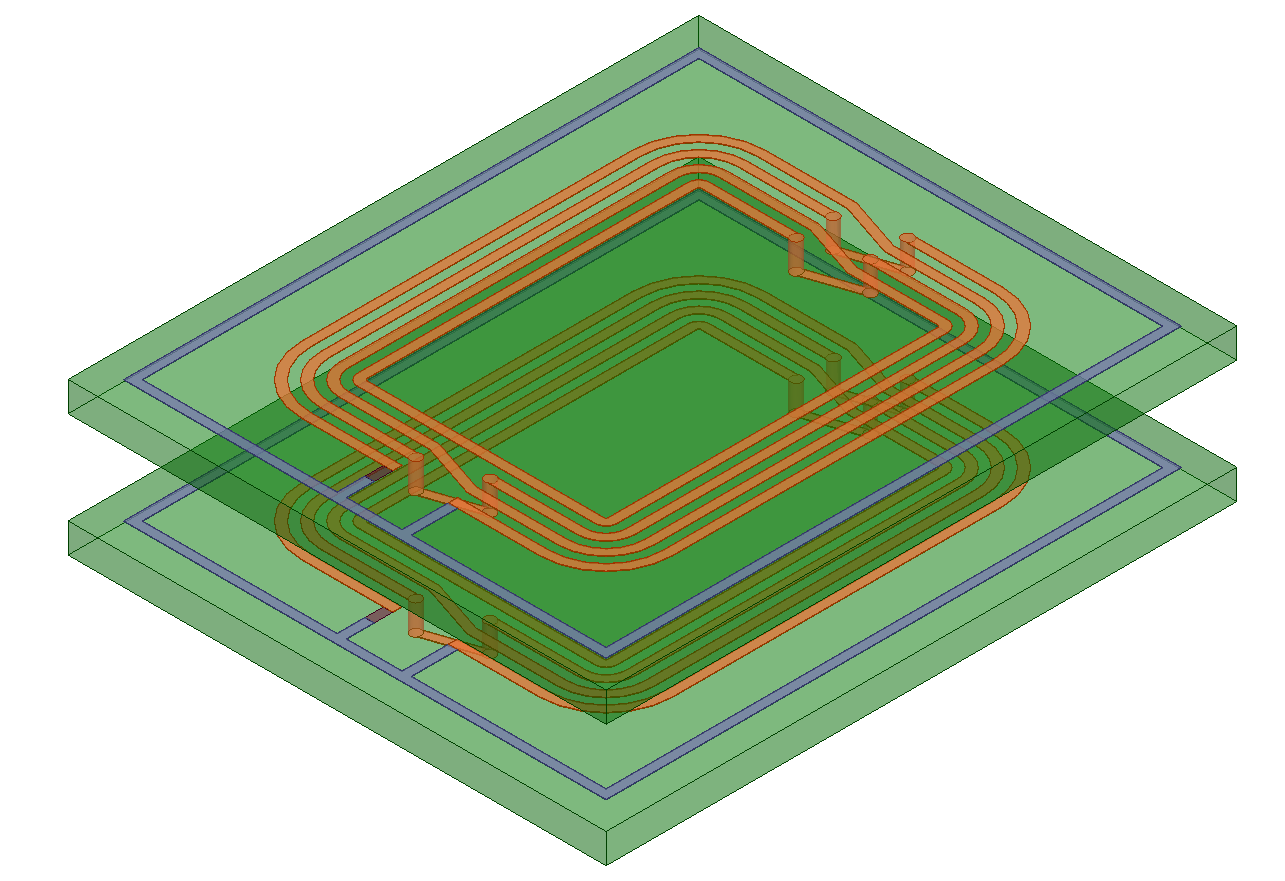
\includegraphics[width=.49\textwidth]{img/ant_couple.png} \label{fig:ant_couple_model}}
\hfill
 \subfloat[Equivalent schematic]  {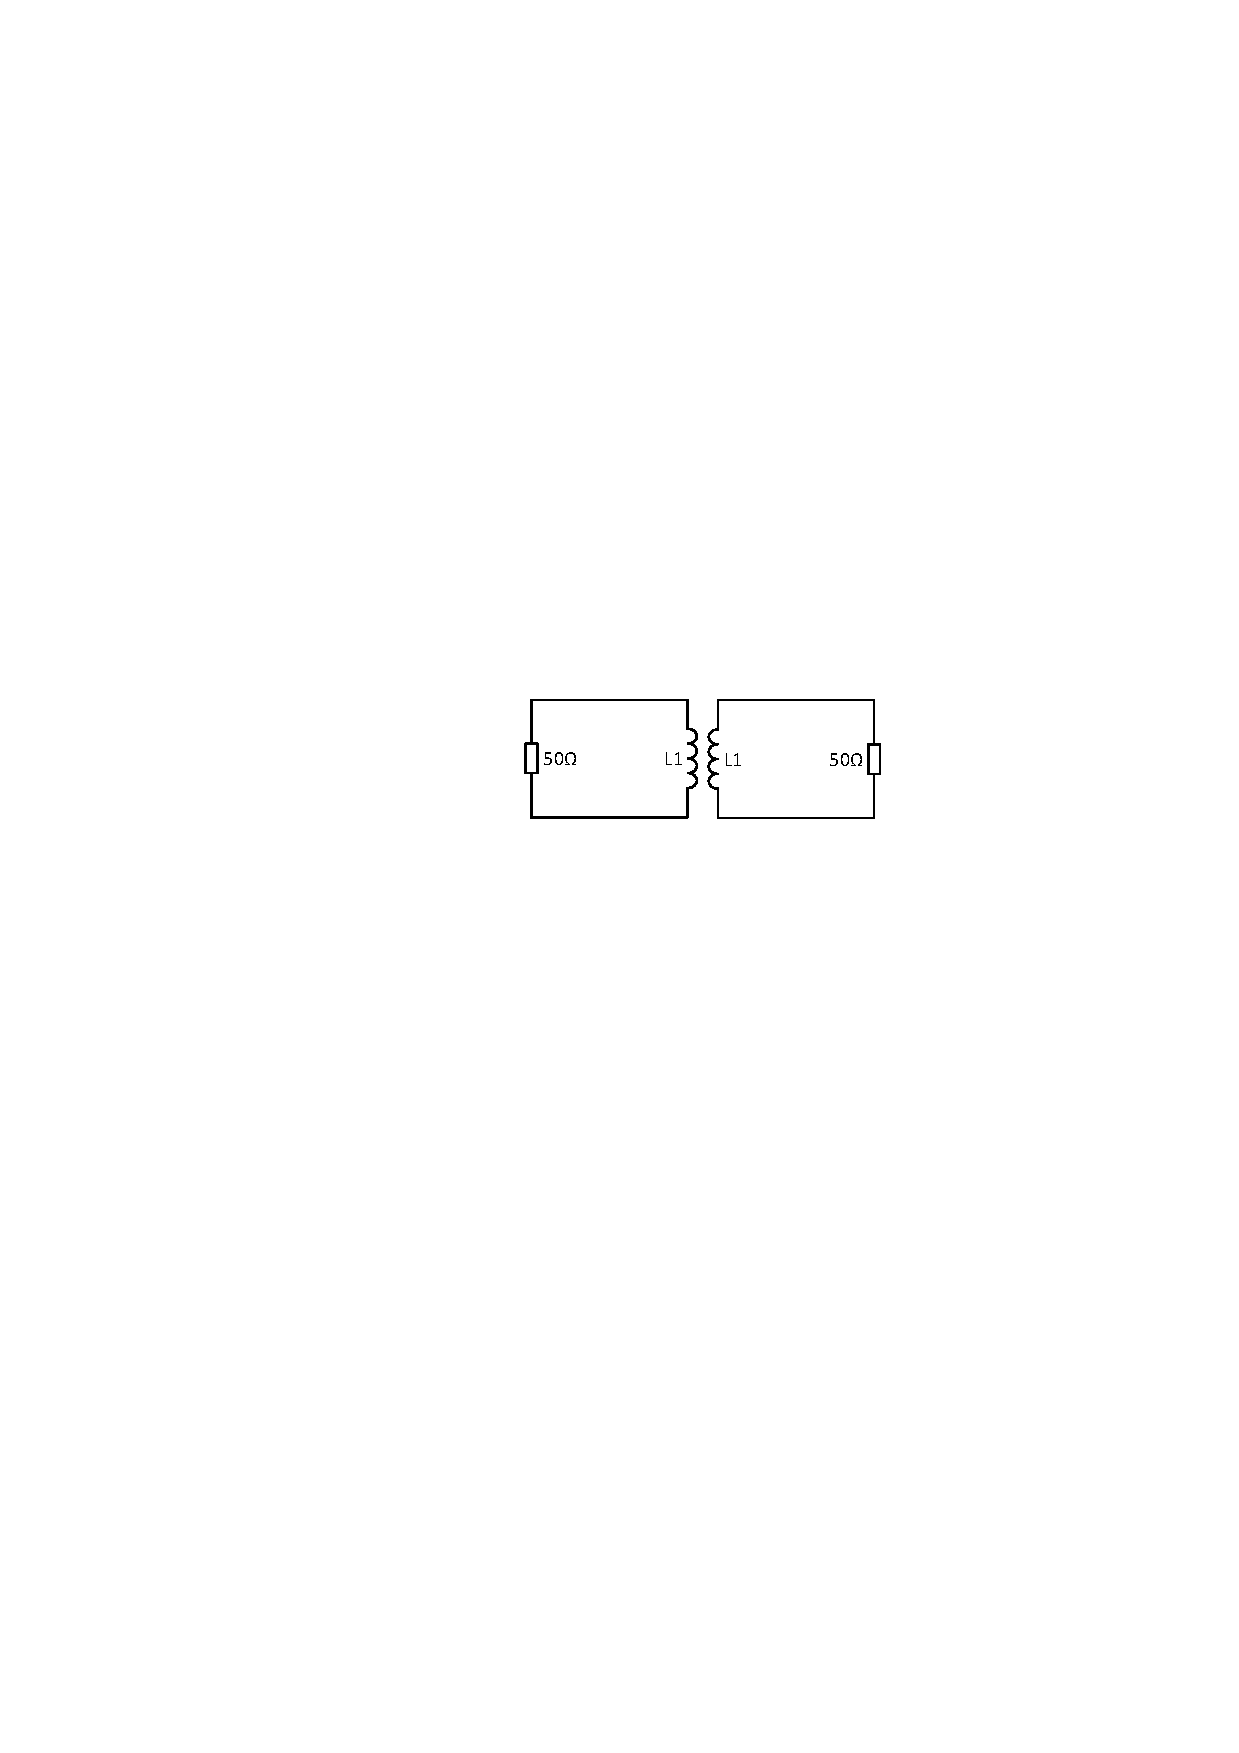
\includegraphics[width=.49\textwidth]{img/ant_couple.pdf}\label{fig:ant_couple_schematic}}
 \caption{Antenna coupling model} 
\label{fig:ant_couple} 
\end{figure}

\begin{table}[H]
\caption{Coupling parameters for varying coils distance} 
\begin{center}
\begin{tabular}{c|c|c|c|c}
\hline \hline
Parameter 	& 1 mm	& 5 mm 	& 10 mm	 & \si{\milli\meter}\\ \hline
L1		& -	& -	& -	 & \si{\nano\henry} \\ \hline
L2		& -	& -	& -	 & \si{\nano\henry} \\ \hline
L12		& -	& -	& -	 & \si{\nano\henry} \\ \hline
k		& -	& -	& -	 & -		    \\ \hline
Q		& -	& -	& -	 & -		    \\
\hline \hline
\end{tabular}
\end{center}
\label{tab:ant_couple_parameter}
\end{table}%


The power transfer efficiency of the physical link created by coupled coils is very important. [CITE] states 
that efficiency depends k of coupling system and Q of coil and hence high k and high Q is always desirable and obviously coil optimisation 
is the most important part of coupling system design. \cite{ant_optimal_resonance} and \cite{ant_PSC_geometry} discusses some techiques to 
optimise transfer efficiency of inductive link: \cite{ant_optimal_resonance} about matching the load for better resonance whereas 
\cite{ant_PSC_geometry} about designing optimal coil geometry for higher Q. The former one compares the efficiency of general inductive coupling 
and conventional resonant coupling and their limitation in achieving higher effieicncy. This eventually proposes 
optimal resonant load transformation which has better immunity to poor coupling and load variation. Likewise, the later one 
describes step by step iterative process of designing an antenna with optimal geometry for the given 
design constraints. \\


In this project, conventional resonance coupling as in [CITE] is implemented to tune both primary and secondary 
to the power career frequency. This method makes the bandwidth narrower but increase Q at operating frequcncy, 
making gain maximum at this desired frequency. \\


For the purpose of making a resonanat inductive link, the S parameter of coupled antenna system in HFSS 
is exported to ADS in order to design matching networks using capacitors only. Impedance of  primary antenna is 
mathched to 50 \si{\ohm} source resistance and impedance of secondary is matched to load impedance (50 \si{\ohm} load or input 
impedance chip(?)) as shown in \ref{fig:ant_couple_resonant}. $Cp1$ and $Cp2$ together with $L1$ created parallel resonant circuit 
on the primary side and $Cs1$ together with $L2$ creates the secondary resonant circuit at 13.56 MHz, a pair of
 Lc tanke circuit si thus made tunned at same frequency. Resonant coupling system with 5 mm separation is taken as a typical example. The losses at both the terminals for this case 
just around our operating frequency are as shown in figure \ref{fig:ant_S_loss}. These plots show that power 
losses at both the ports have been reduced by at least an order of magnitude.

\begin{figure}[!htbp] %figure placement: here, top, bottom, or page
   \centering
   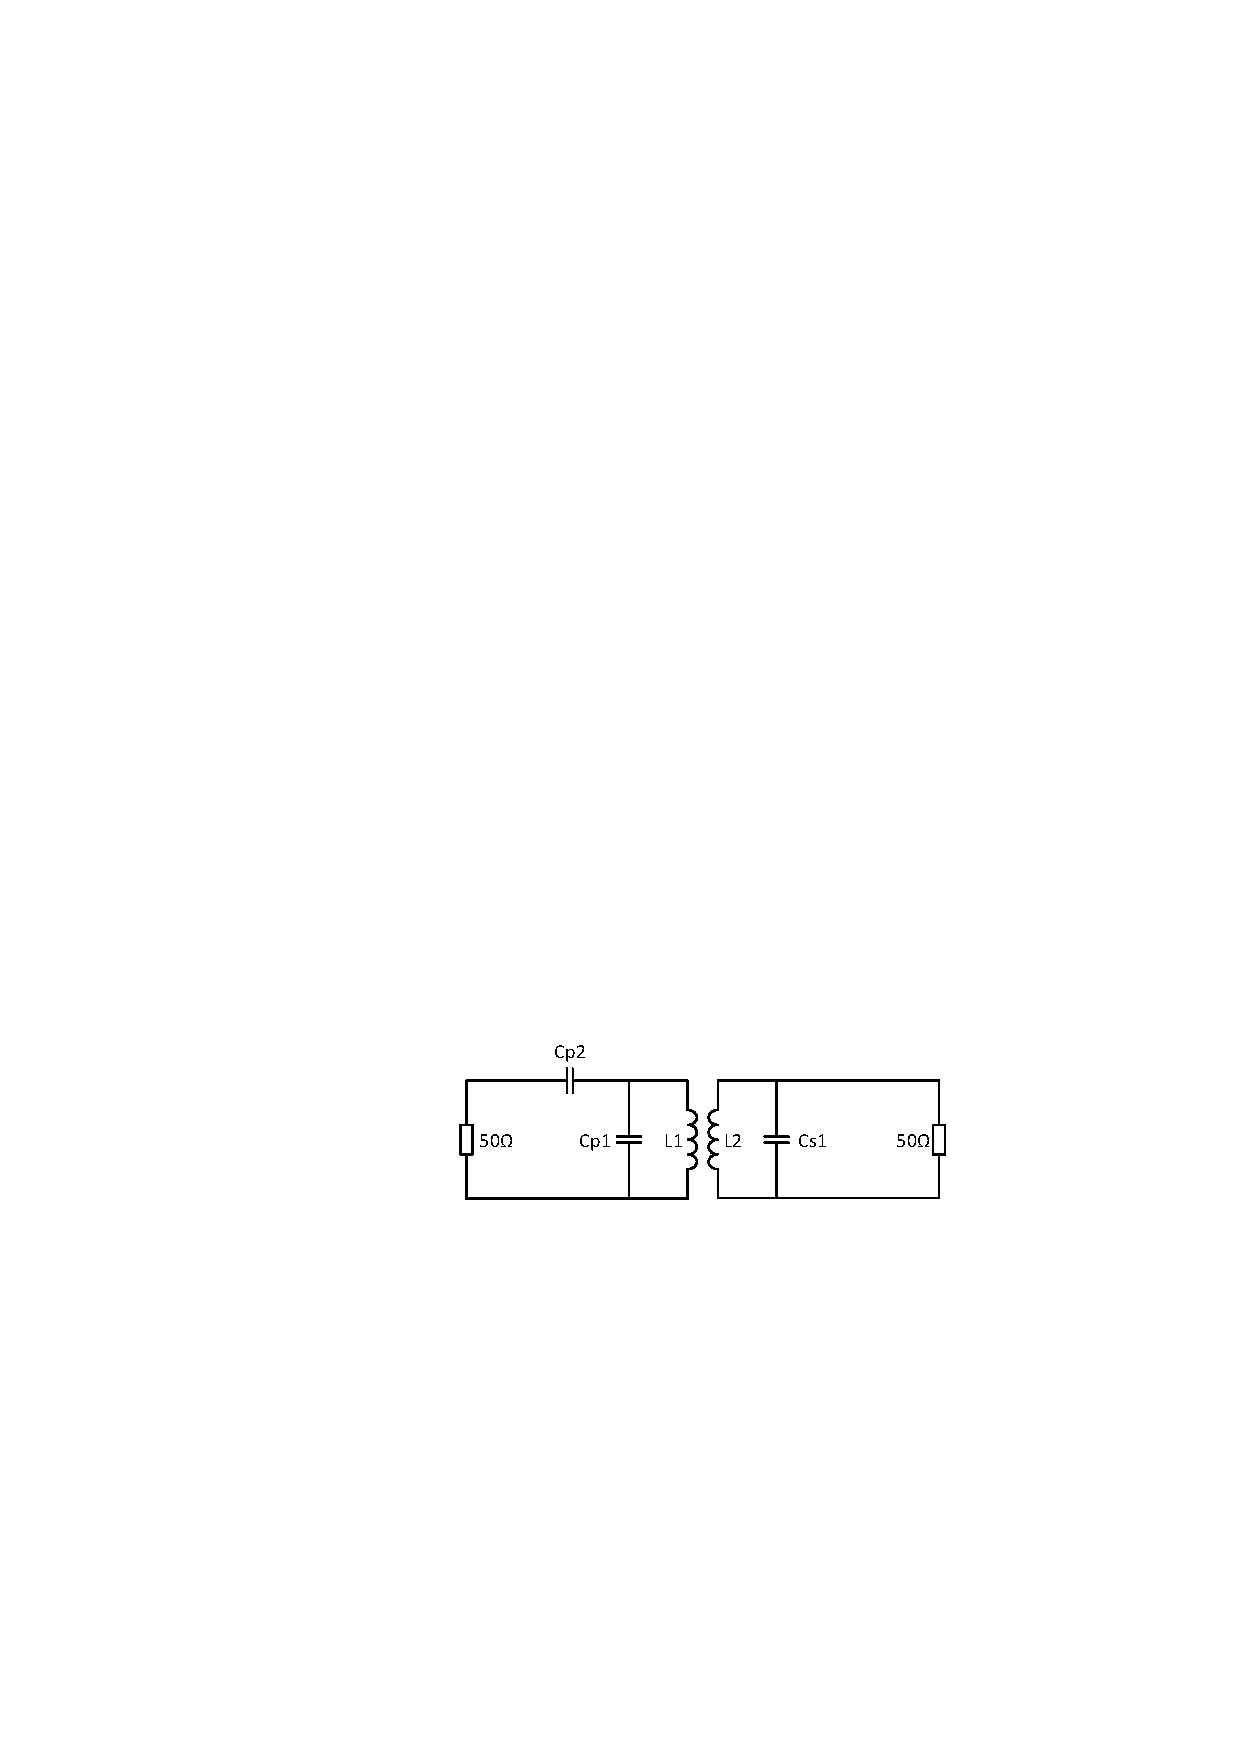
\includegraphics[width=0.8\textwidth]{img/ant_couple_resonant.pdf} 
   \caption{Resonant coupled inductive link}
   \label{fig:ant_couple_resonant}
\end{figure}

\begin{figure} [!htbp]
  \centering
  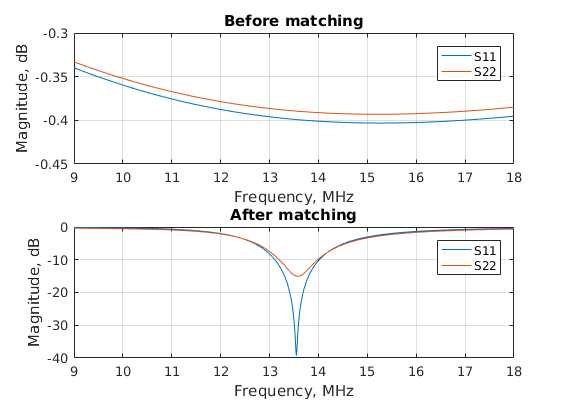
\includegraphics[width=0.9\textwidth]{img/ant_S_loss.png} 
 \caption{Power loss before and after matching} 
\label{fig:ant_S_loss} 
\end{figure}


The  vlaues of  s11 and s22   for coupled link before and after resonance is listed in [table]. 

 
\clearpage
\newpage
\nocite{*}
\printbibliography

\newpage
\listoffigures

\newpage
\listoftables

%\printindex
\newpage
\printnoidxglossaries

\end{document}